\documentclass[12pt,a4paper,UTF8]{ctexart}
\usepackage{geometry}
	\geometry{left=2.5cm,right=2.5cm,top=2cm,bottom=2cm}
\usepackage{xeCJK,amsmath,paralist,enumitem,booktabs,multirow,graphicx,subfig,setspace}
	\setlength{\parindent}{2em}
\usepackage[colorlinks,linkcolor=blue,urlcolor=blue]{hyperref}

%%%%%%%%%%%%%%%%%%%%%%%%%正文开始%%%%%%%%%%%%%%%%%%%%%%%%%%
\begin{document}

\title{\vspace{-2cm}\LARGE\bfseries C3.1 基于OMA的原子发射光谱测量\footnotemark[1]}
\author{\large\textit{黄子维}$^{1}$\footnotemark[2],\large\textit{黄睿杰}$^{2}$\footnotemark[3] \\ 
\small{1,2 \textit{中山大学 中山医学院,广东 广州 }510275}}
\date{}
\maketitle
\setcounter{page}{0}
\thispagestyle{empty}
\vspace{-1.5em}
\begin{spacing}{2.0}
{\bfseries 摘 {} 要:}
玻尔原子模型指出,当原子从一种定态跃迁到另一种定态时,将辐射或吸收一定频率的光子,光子的能量由这两个定态的能量差决定。
这一发现成功解释了氢原子光谱的不连续性,为量子理论的发展奠定了基础,同时该发现在物质组分和结构分析领域也有着重要应用。
对原子发射光谱的精密测量是理解原子跃迁过程的物理基础,本实验中,我们采用基于反射光栅的光学多道分析仪(OMA)测量原子发射光谱。

我们扫描了九种实验室常用光源(汞灯,钠灯,氢氘灯,溴钨灯和五种颜色的LED灯)的原子发射光谱(如图\ref{fig:0}),
发现其中汞灯,钠灯和氢氘灯光谱为分立谱,而溴钨灯和五种颜色LED灯光谱为连续谱。
接下来,对于分立谱光源,我们使用测量得到的汞灯谱线与标准谱线对比得到标定关系,并据此标定了其他谱线,
同时我们基于在更小光栅距离下测量得到的钠灯光谱,研究了钠双黄线的特征。
最后,对于连续谱光源,我们使用高斯函数插值计算LED灯的波包中心波长及其半高宽,并研究了溴钨灯光源的光谱特点。
\begin{figure}[htbp]
	\centering
	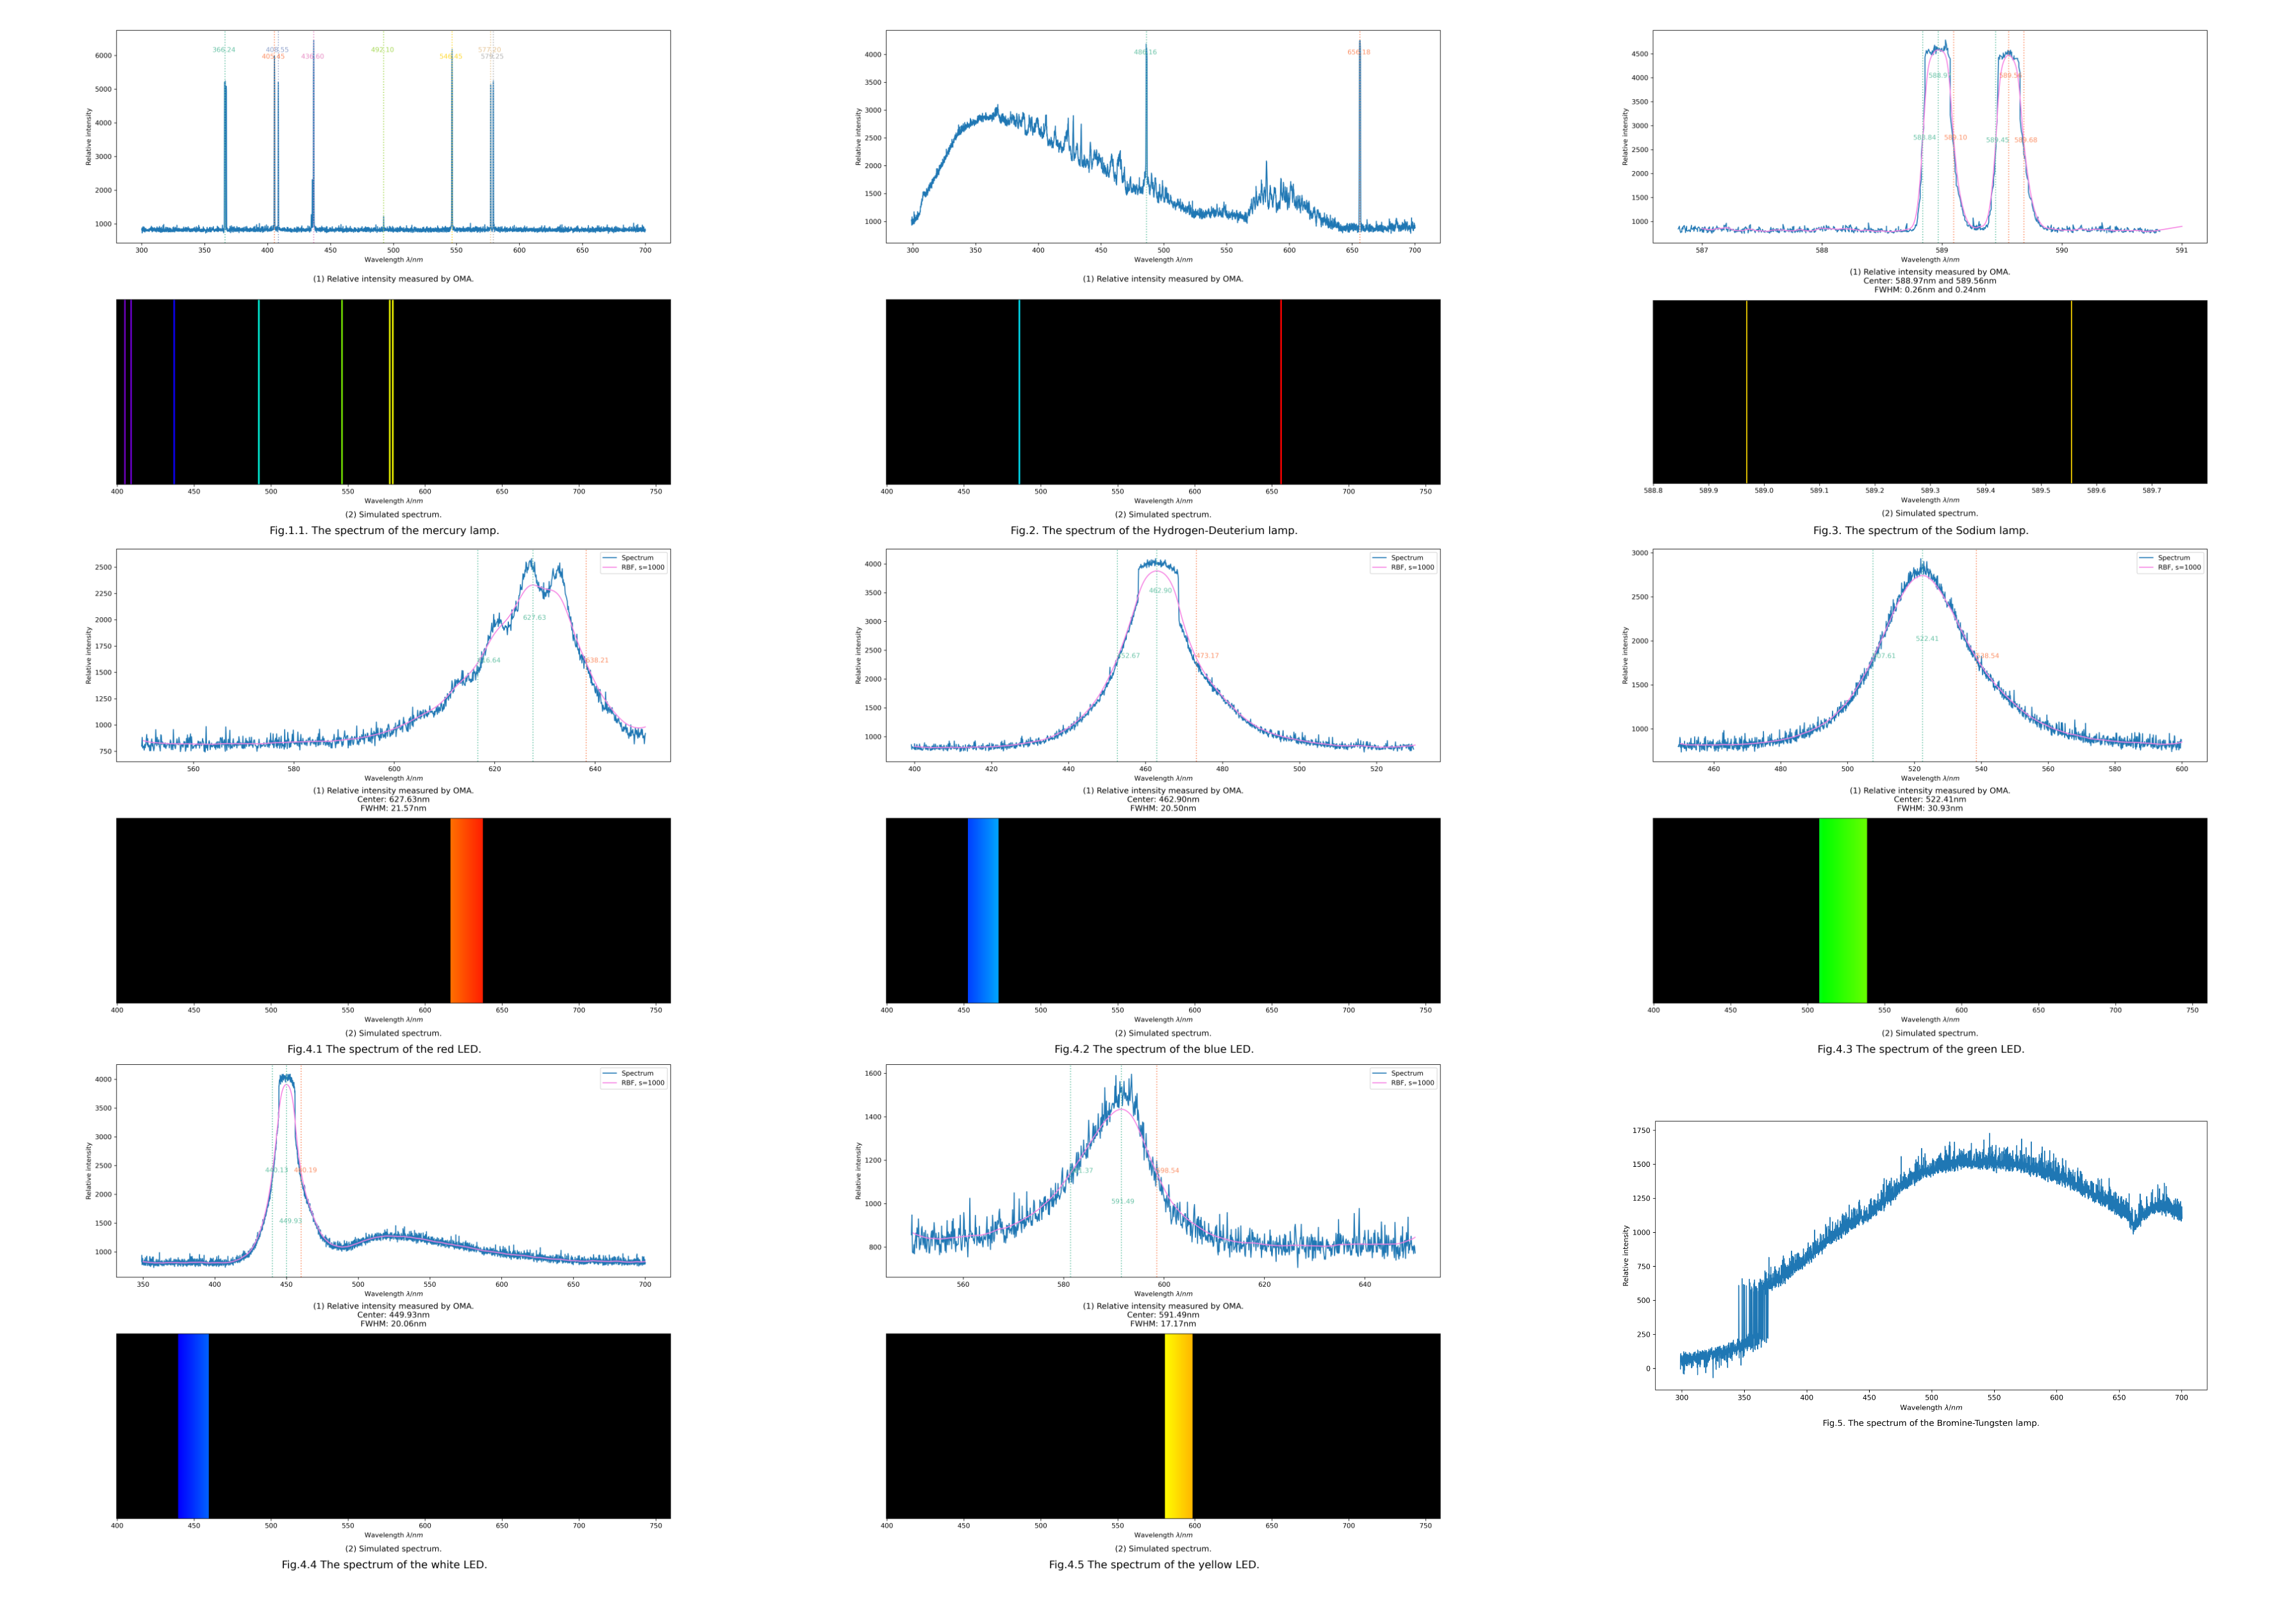
\includegraphics[width=0.55\textwidth]{attachments/Fig.0.png}
	\caption{实验室常用光源的原子发射光谱}
	\label{fig:0}
\end{figure}
\par
\vspace{-0.5em}
\bfseries{关键词}: 光学多道分析仪(OMA),原子发射光谱
\vspace{0.5em}
\end{spacing}

\renewcommand{\thefootnote}{\fnsymbol{footnote}}
\footnotetext[1]{由中山大学物理学院陆佑堂提供器材和指导。}
\footnotetext[2]{通信作者,20980066,\url{huangzw29@mail2.sysu.edu.cn}}
\footnotetext[3]{实验参与人,20980062}

%%%%%%%%附录:数据处理%%%%%%%
\newpage
\pagestyle{plain}
\begin{center}
\LARGE\textbf{实验C3.1 原子发射光谱}
\end{center}

%%信息
\begin{doublespacing}
	\centering
	\begin{tabular}{ll}
	 & \\
	{\CJKfontspec{Droid Sans Fallback} 实验人:黄子维 20980066} & {\CJKfontspec{Droid Sans Fallback}合作者:黄睿杰 20980062}\\
	{\CJKfontspec{Droid Sans Fallback} 实验时间:2021.10.9~星期六~上午} & {\CJKfontspec{Droid Sans Fallback} 室温:23$^{\circ}$C~相对湿度:72\%}
	\end{tabular}
\end{doublespacing}
\subsection*{【实验参数】}
除钠灯外,其余光谱均在光栅间隔0.1nm,时间间隔0.1s下测量。钠灯光谱光栅间隔0.005nm,时间间隔0.01s。

钠双黄线和LED灯光谱拟合方法为高斯函数插值(Radial basis function interpolation, Rbf),光滑度设置为1000。

\subsection*{【数据处理及分析】}
\subsubsection*{1. 汞灯谱线及标定}
使用OMA测量得到的汞灯谱线及可见光范围内谱线的模拟光谱如图\ref{fig:1.1}所示。
测量得到谱线波长如表\ref{tab:1.1}。

\begin{figure}[htbp]
	\centering
	\subfloat[汞灯谱线测量值]{\label{fig:1.1}
	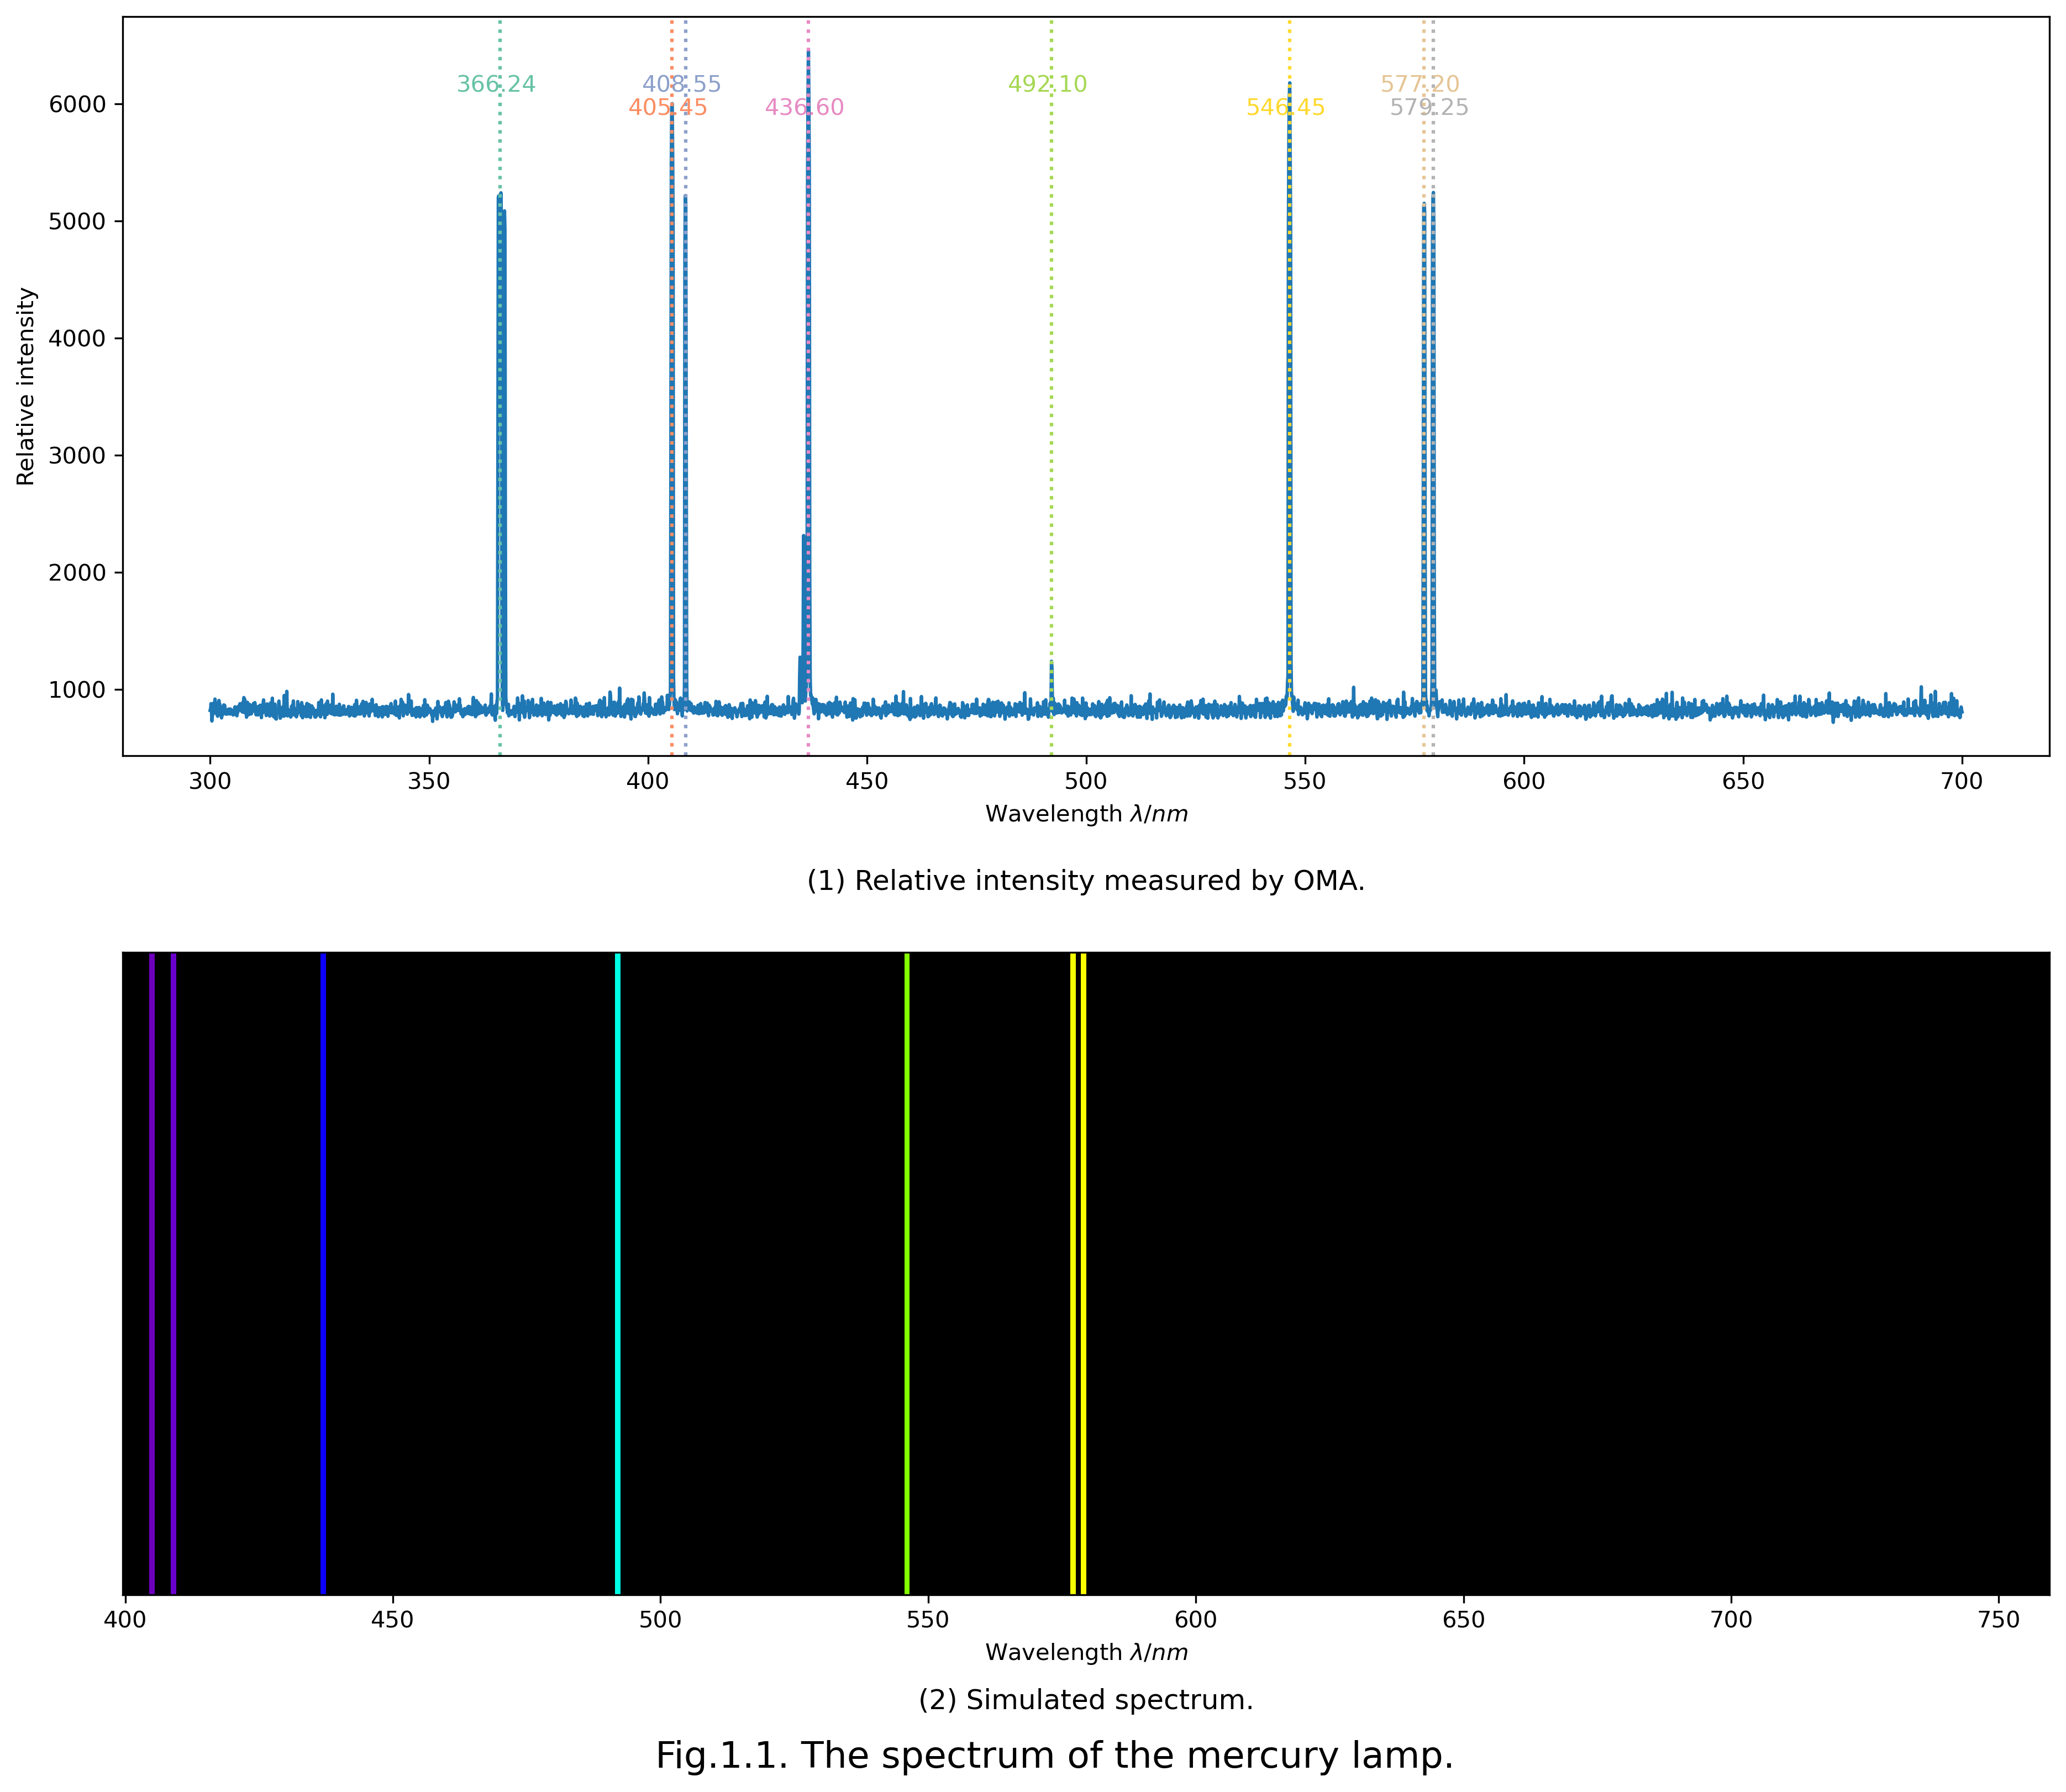
\includegraphics[width=0.55\textwidth]{attachments/Fig.1.1.png}
	}
	\subfloat[使用汞原子标准谱线标定光谱]{\label{fig:1.2}
	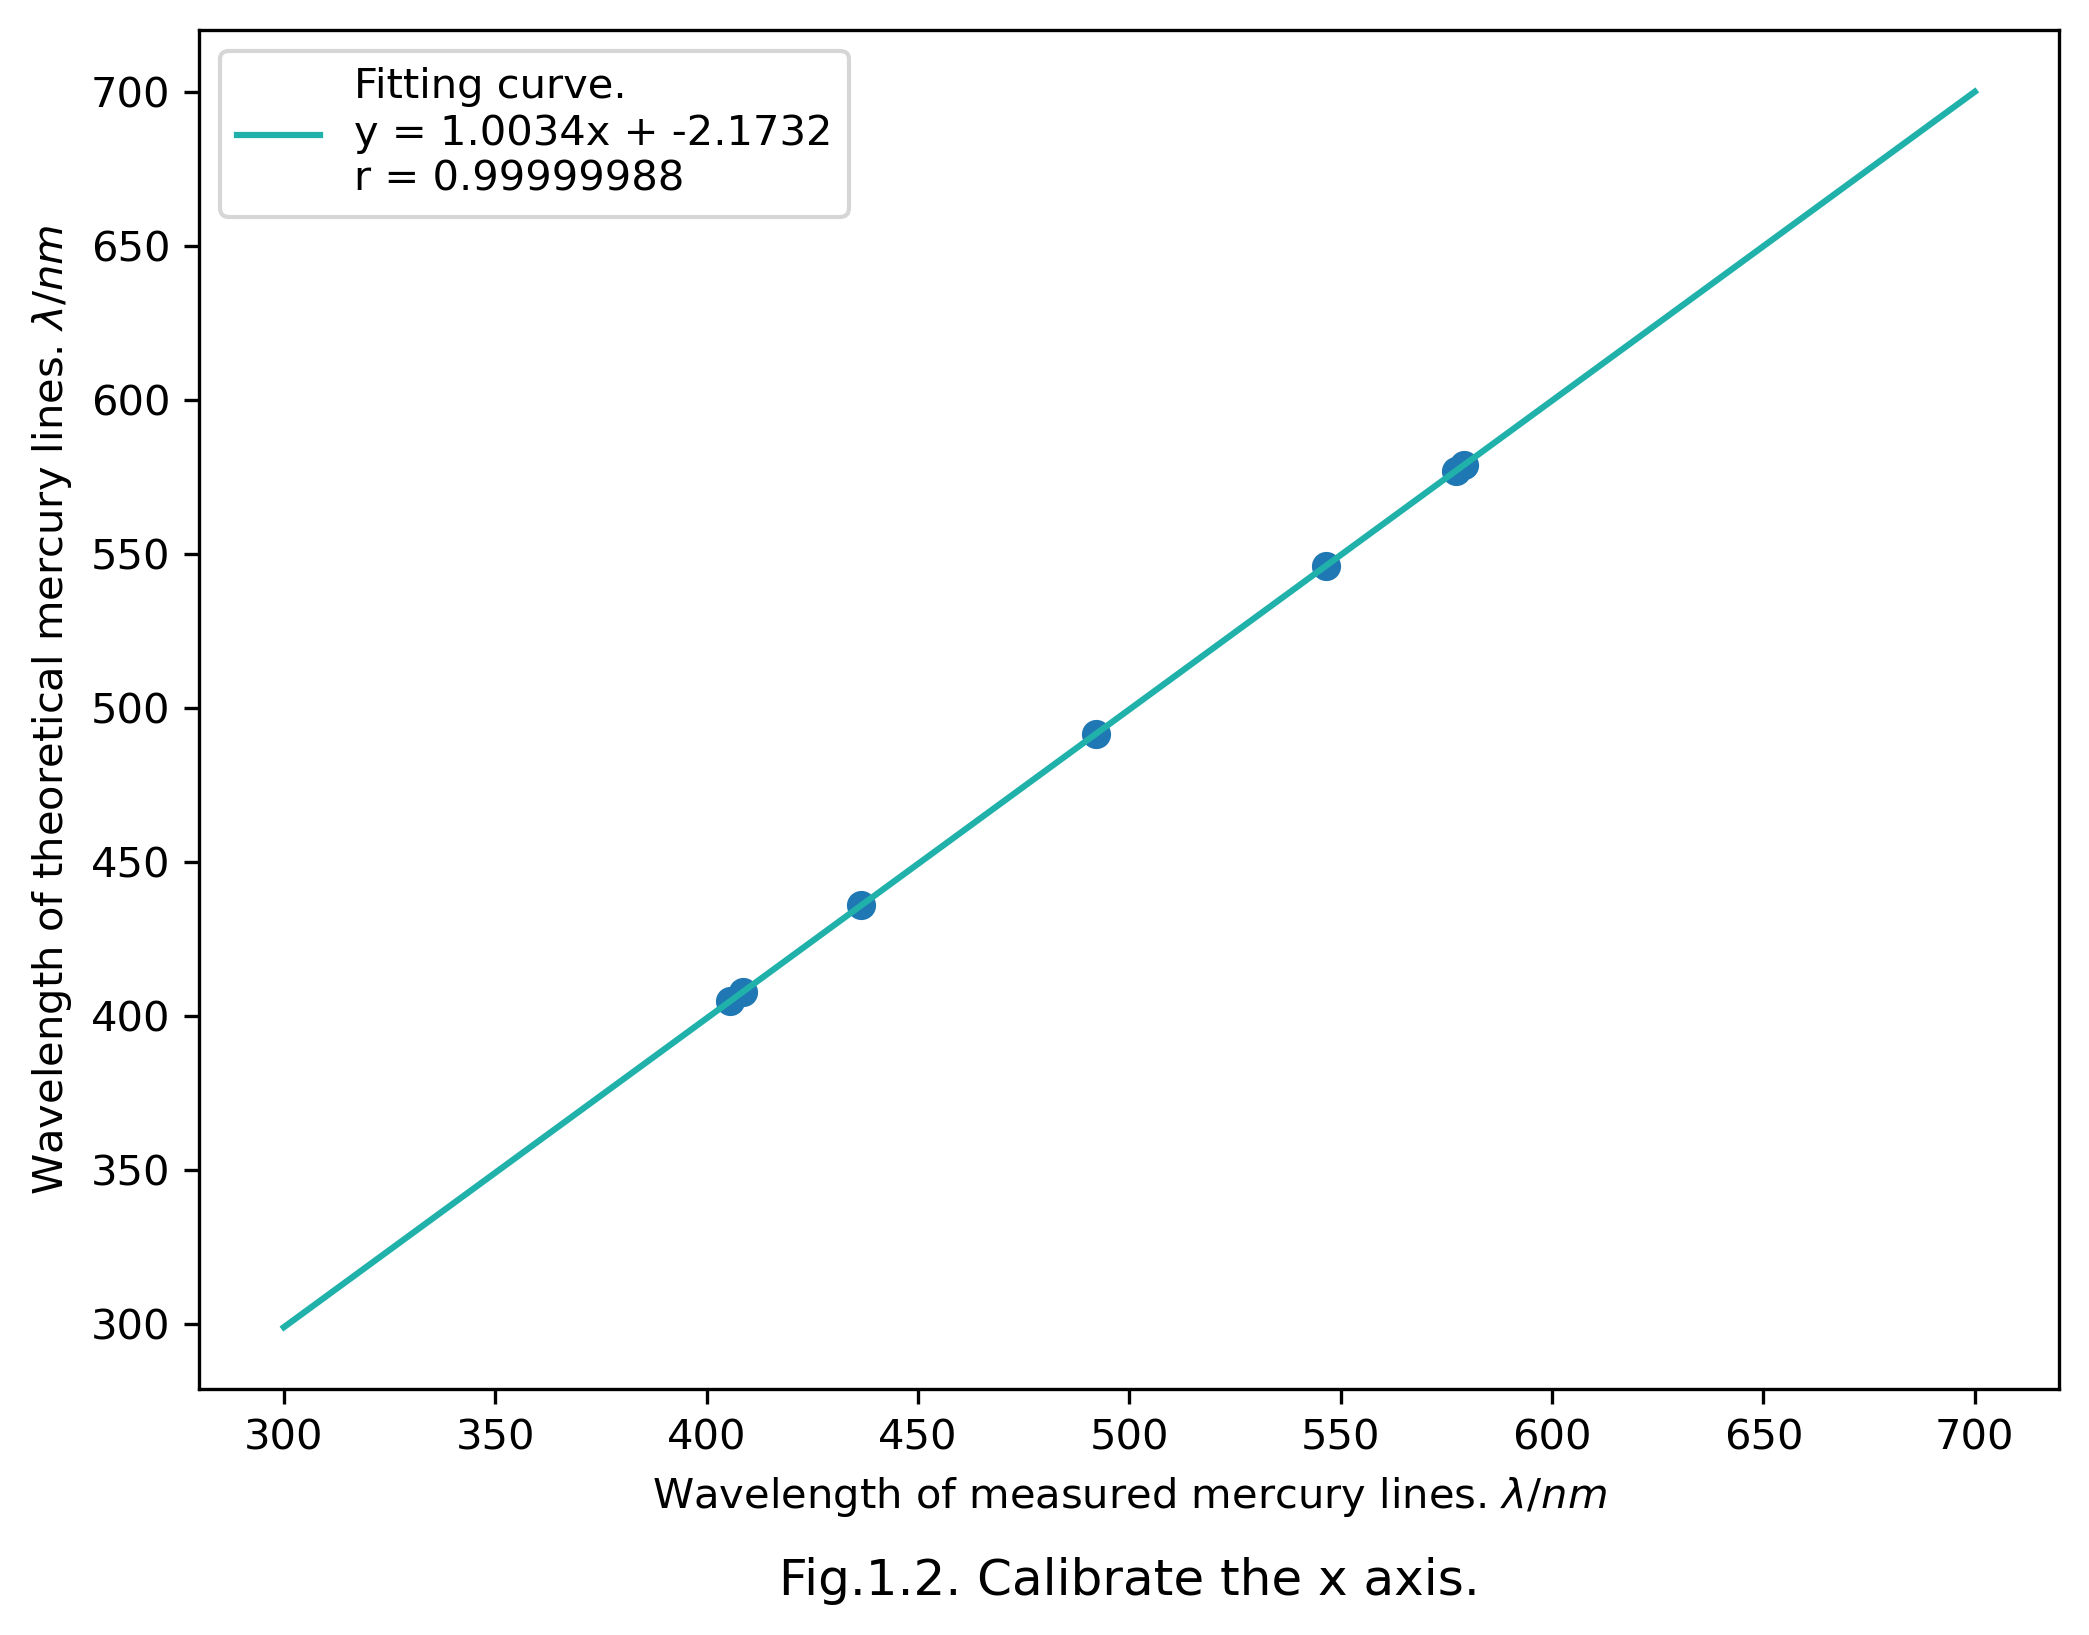
\includegraphics[width=0.45\textwidth]{attachments/Fig.1.2.png}
	}
	\caption{汞灯光谱}
\end{figure}

\begin{table}[htbp]
	\centering
	\begin{tabular}{ccccccccc}
	\toprule
	波长/nm &$366.24$ &$405.45$ &$408.55$ &$436.60$ &$492.10$ &$546.45$ &$577.20$ &$579.25$\\
	\midrule
	颜色 &/ &Purple &Purple &Blue &Cyan &Green &Yellow &Yellow \\
	\bottomrule
    \end{tabular}
	\caption{\textbf{汞灯谱线测量值}}
	\label{tab:1.1}
\end{table}
	
可以看出,汞灯光谱为分立谱。其中,除了波长为$366.24nm$谱线在紫外区外,其余谱线均在可见光区。
光谱在$405.nm$和$577nm$附近存在双线现象,波长为$492.10nm$谱线相对强度较弱。

使用测量得到的汞灯光谱与汞灯标准光谱(数据来源:\href{http://hyperphysics.phy-astr.gsu.edu/hbase/quantum/atspect2.html#c2}{Mercury spectrum | Hyperphysics@GSU})对比(如表\ref{tab:1.2}),
得到标定关系(如图\ref{fig:1.2})。使用该标定函数对其余光谱进行标定。如无特殊说明,后续图表的波长值均已标定。
\begin{table}[htbp]
	\centering
	\begin{tabular}{ccccccccc}
	\toprule
	实验值/nm &$405.45$ &$408.55$ &$436.60$ &$492.10$ &$546.45$ &$577.20$ &$579.25$\\
	\midrule
	标准值/nm &$404.656$ &$407.781$ &$435.835$ &$491.604$ &$546.074$ &$576.959$ &$579.065$\\
	\bottomrule
    \end{tabular}
	\caption{\textbf{汞灯谱线测量值}}
	\label{tab:1.2}
\end{table}

\subsubsection*{2. 氢氘灯光谱}
氢氘灯光谱如图\ref{fig:2}所示。测量得到谱线波长如表\ref{tab:2}。

\begin{figure}[htbp]
	\centering
	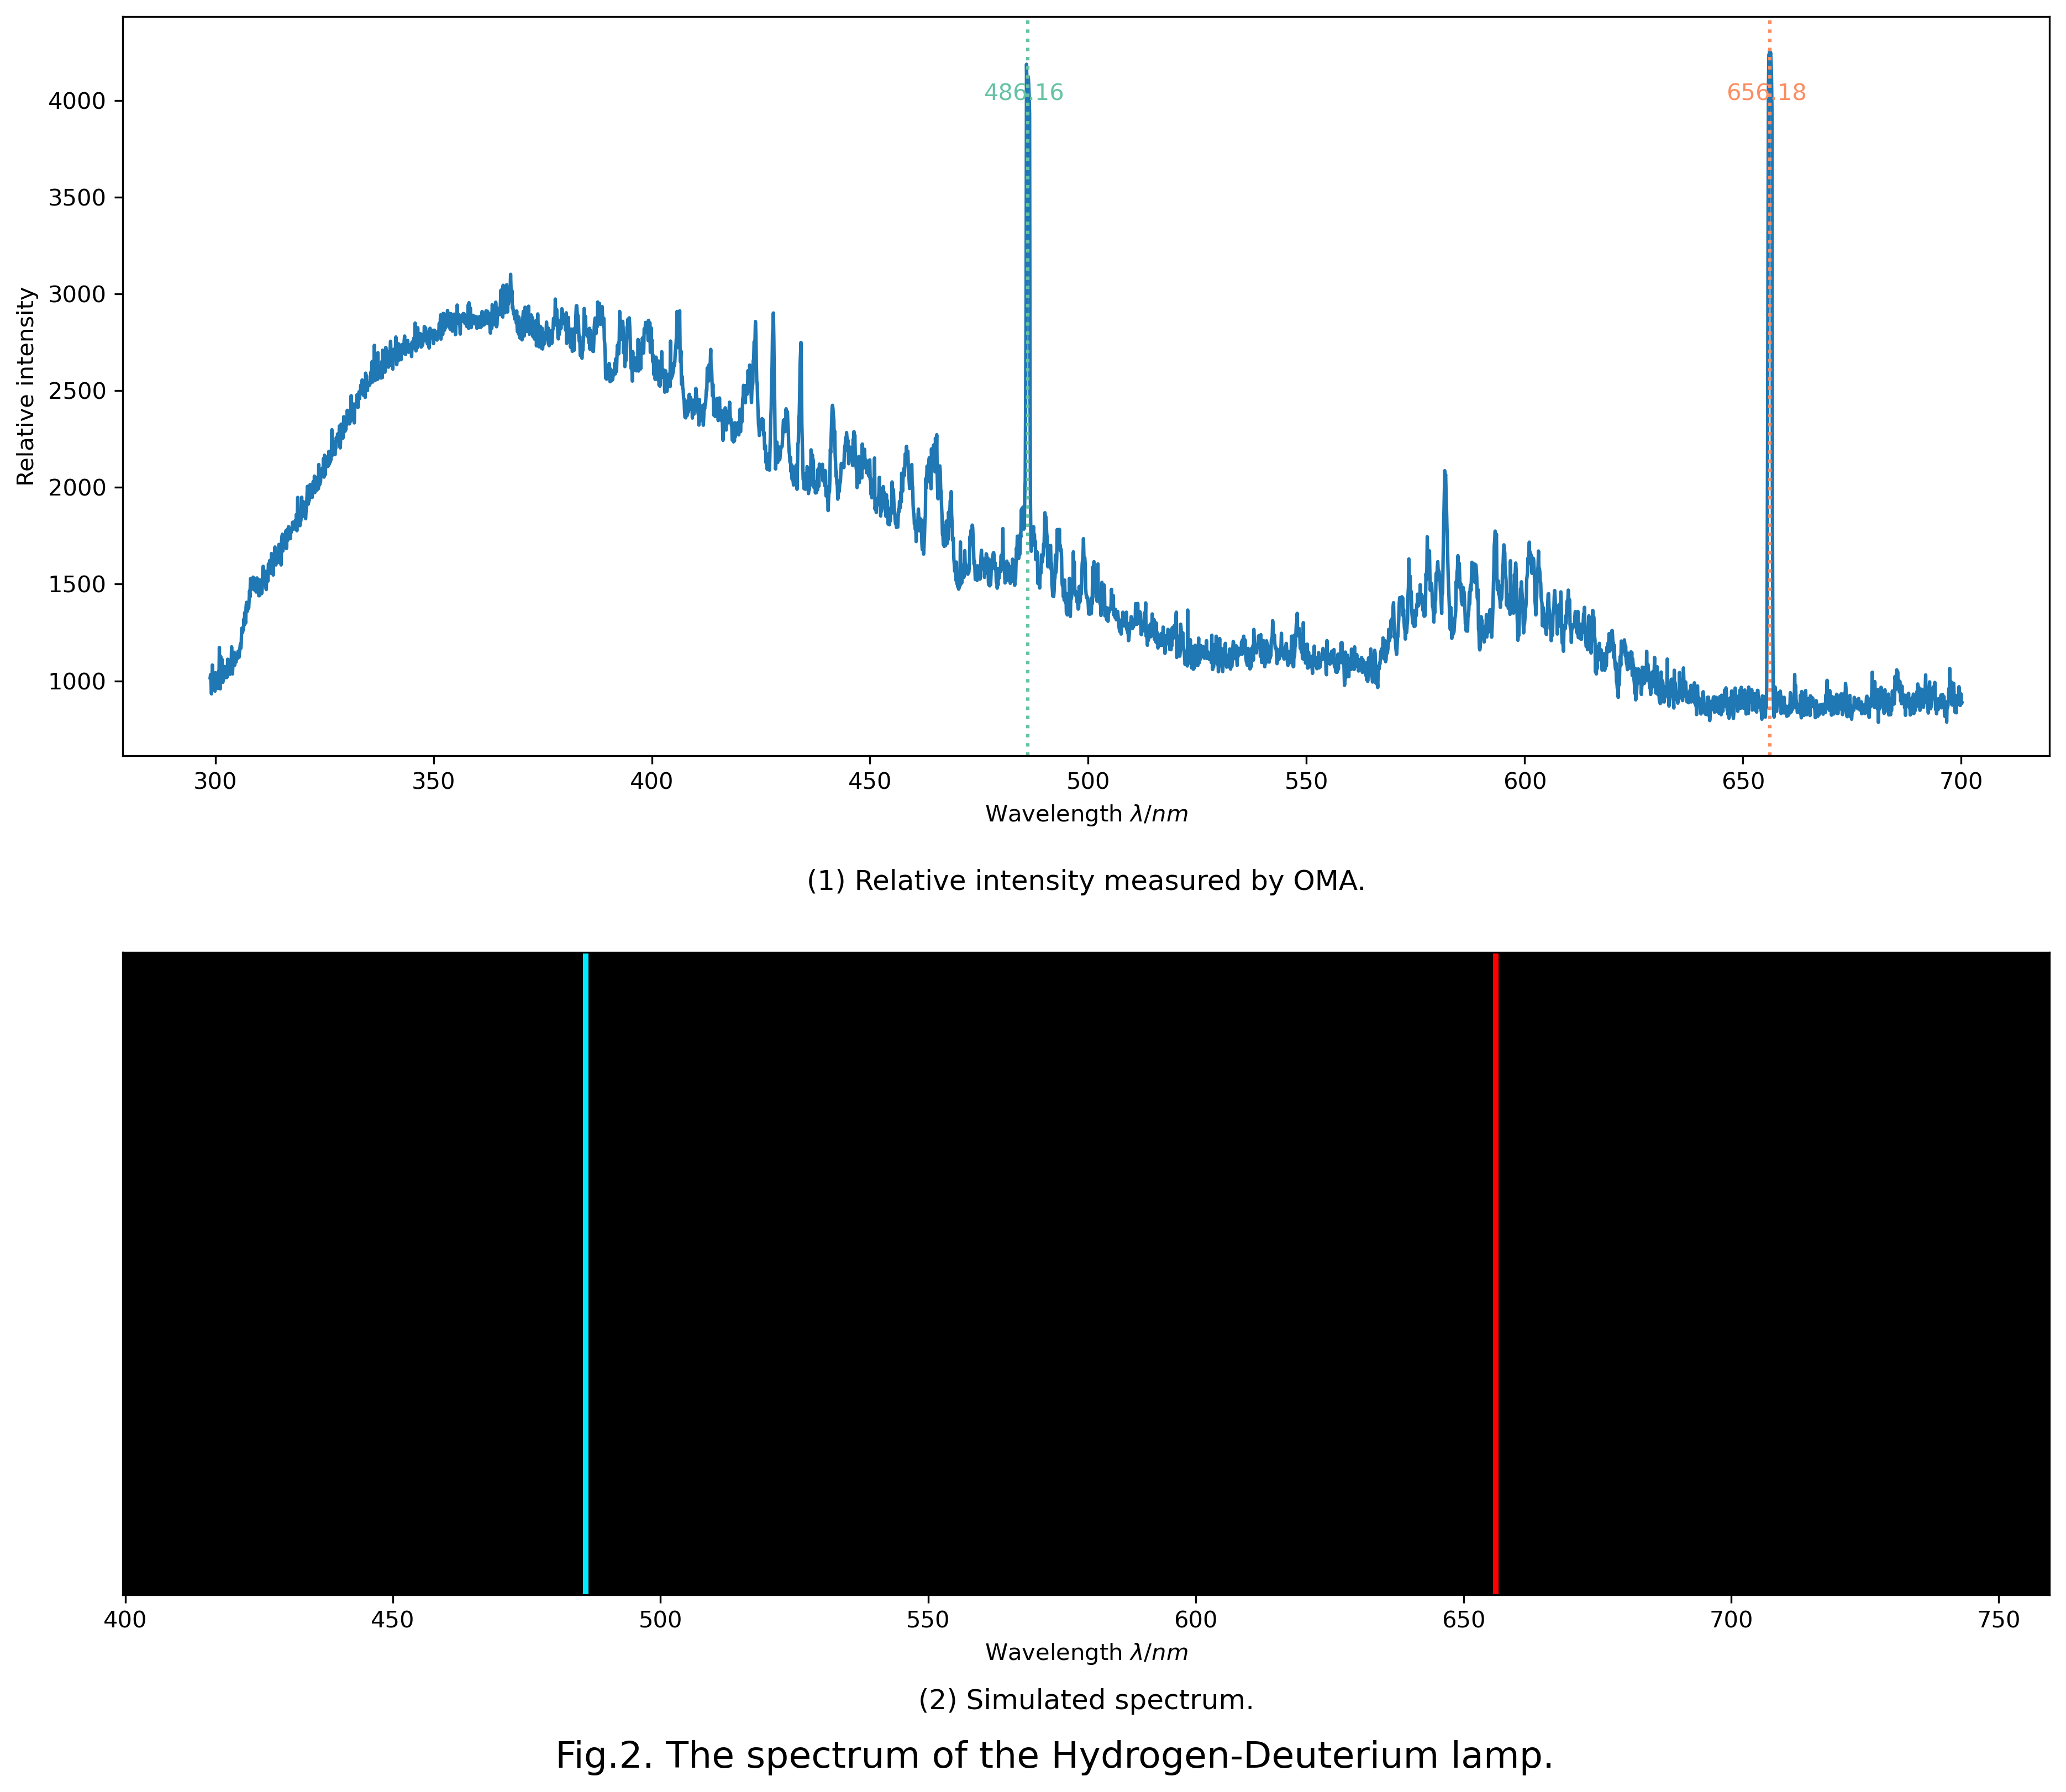
\includegraphics[width=0.8\textwidth]{attachments//Fig.2.png}
	\caption{氢氘灯光谱}
	\label{fig:2}
\end{figure}

\begin{table}[htbp]
	\centering
	\begin{tabular}{ccc}
	\toprule
	波长/nm &$486.16nm$ &$656.18nm$ \\
	\midrule
	颜色 &Cyan &Red  \\
	\bottomrule
    \end{tabular}
    \caption{\textbf{氢氘灯谱线测量值}}
    \label{tab:2}
\end{table}

可以看出,氢氘灯光谱为分立谱,测量得到的谱线均在可见光区,背景光谱存在先上升后下降的趋势。

光谱上未见理论预测的$410.174nm$和$434.047nm$谱线,推测原因是这两条谱线相对强度较小,被掩盖在背景噪声中而无法识别。
此外,理论上$656nm$附近应存在双线$656.272nm$和$656.285nm$,但由于光栅距离较大,分辨率不足,无法识别。

\subsubsection*{3. 钠灯双黄线}
钠灯光谱双黄线如图\ref{fig:3}所示。测量得到谱线中心波长及半高宽如表\ref{tab:3}。

\begin{figure}[htbp]
	\centering
	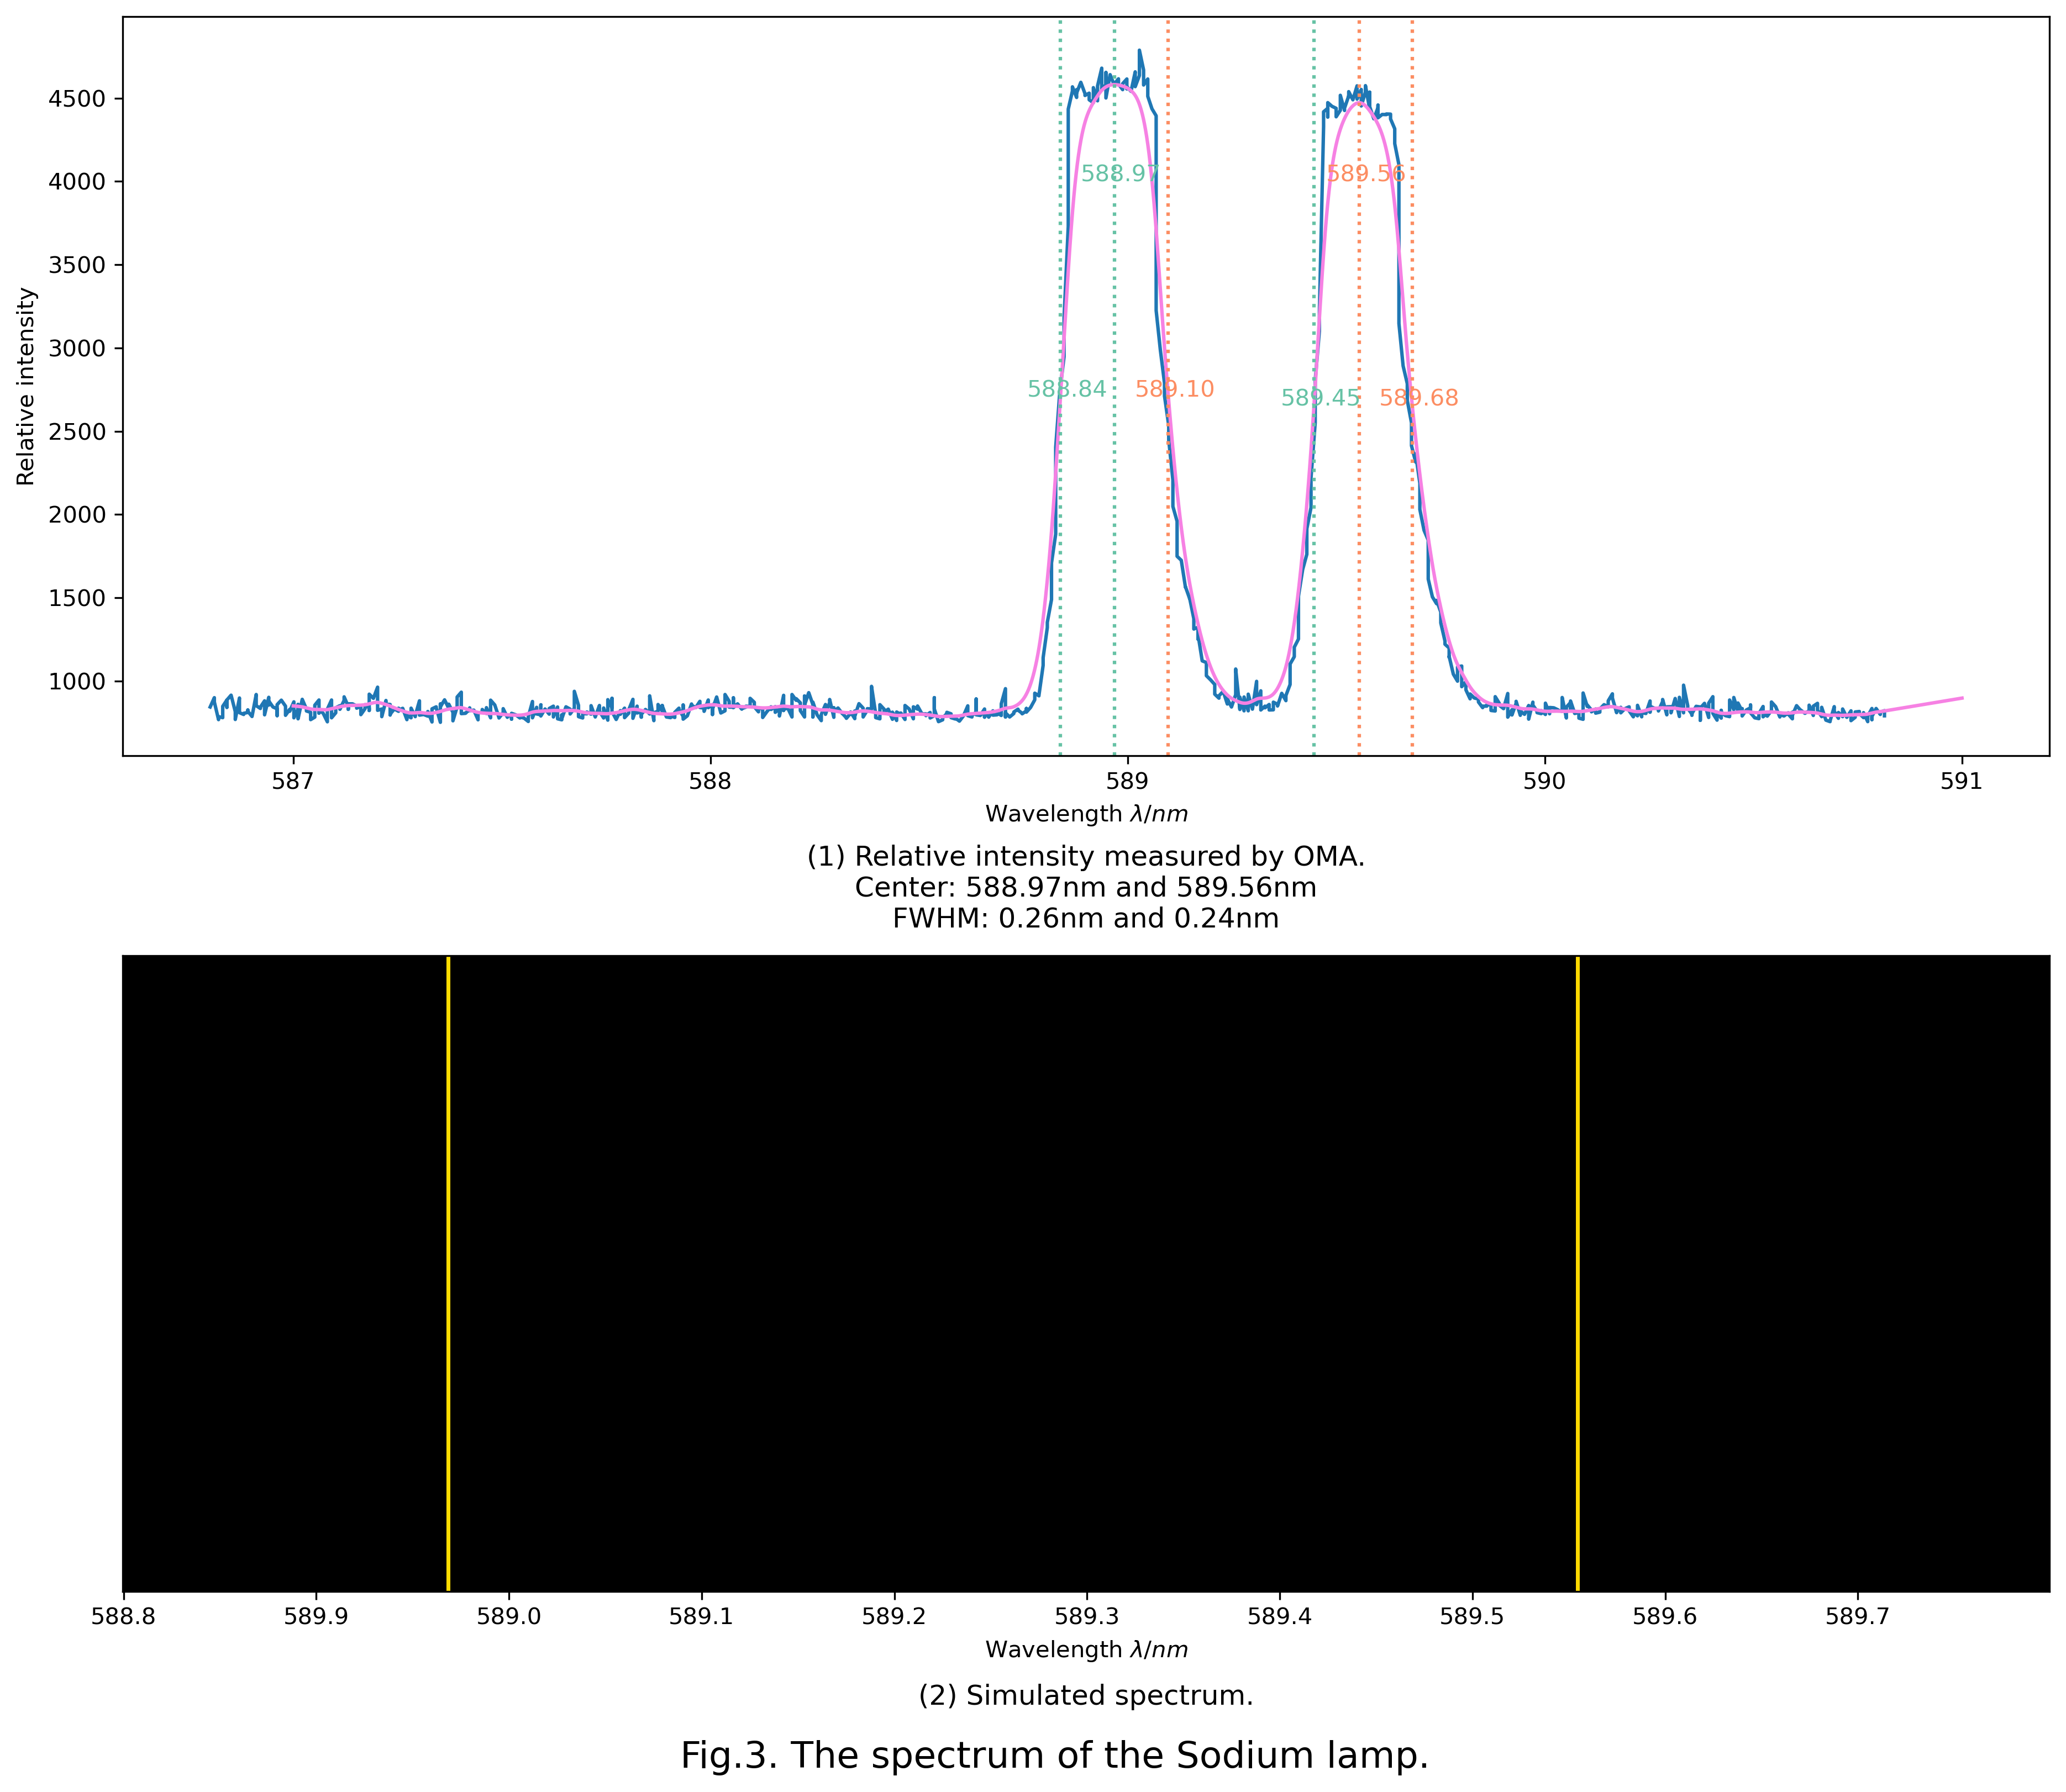
\includegraphics[width=0.8\textwidth]{attachments//Fig.3.png}
	\caption{钠灯双黄线}
	\label{fig:3}
\end{figure}

\begin{table}[htbp]
	\centering
	\begin{tabular}{ccc}
	\toprule
	中心谱线/nm &$588.97$ &$589.56$ \\
	\midrule
	半高宽/nm &$0.26(588.84\sim 589.10)$ &$0.24(589.45\sim 589.68)$  \\
	\bottomrule
    \end{tabular}
	\caption{\textbf{钠灯双黄线}}
    \label{tab:3}
\end{table}

\newpage
\subsubsection*{4. LED灯光谱}
五种颜色的LED的光谱如图\ref{fig:4}所示。各色LED谱线中心波长及半高宽如表\ref{tab:4}。
\begin{figure}[htbp]
	\centering
	\subfloat[Red]{\label{fig:4.1}
	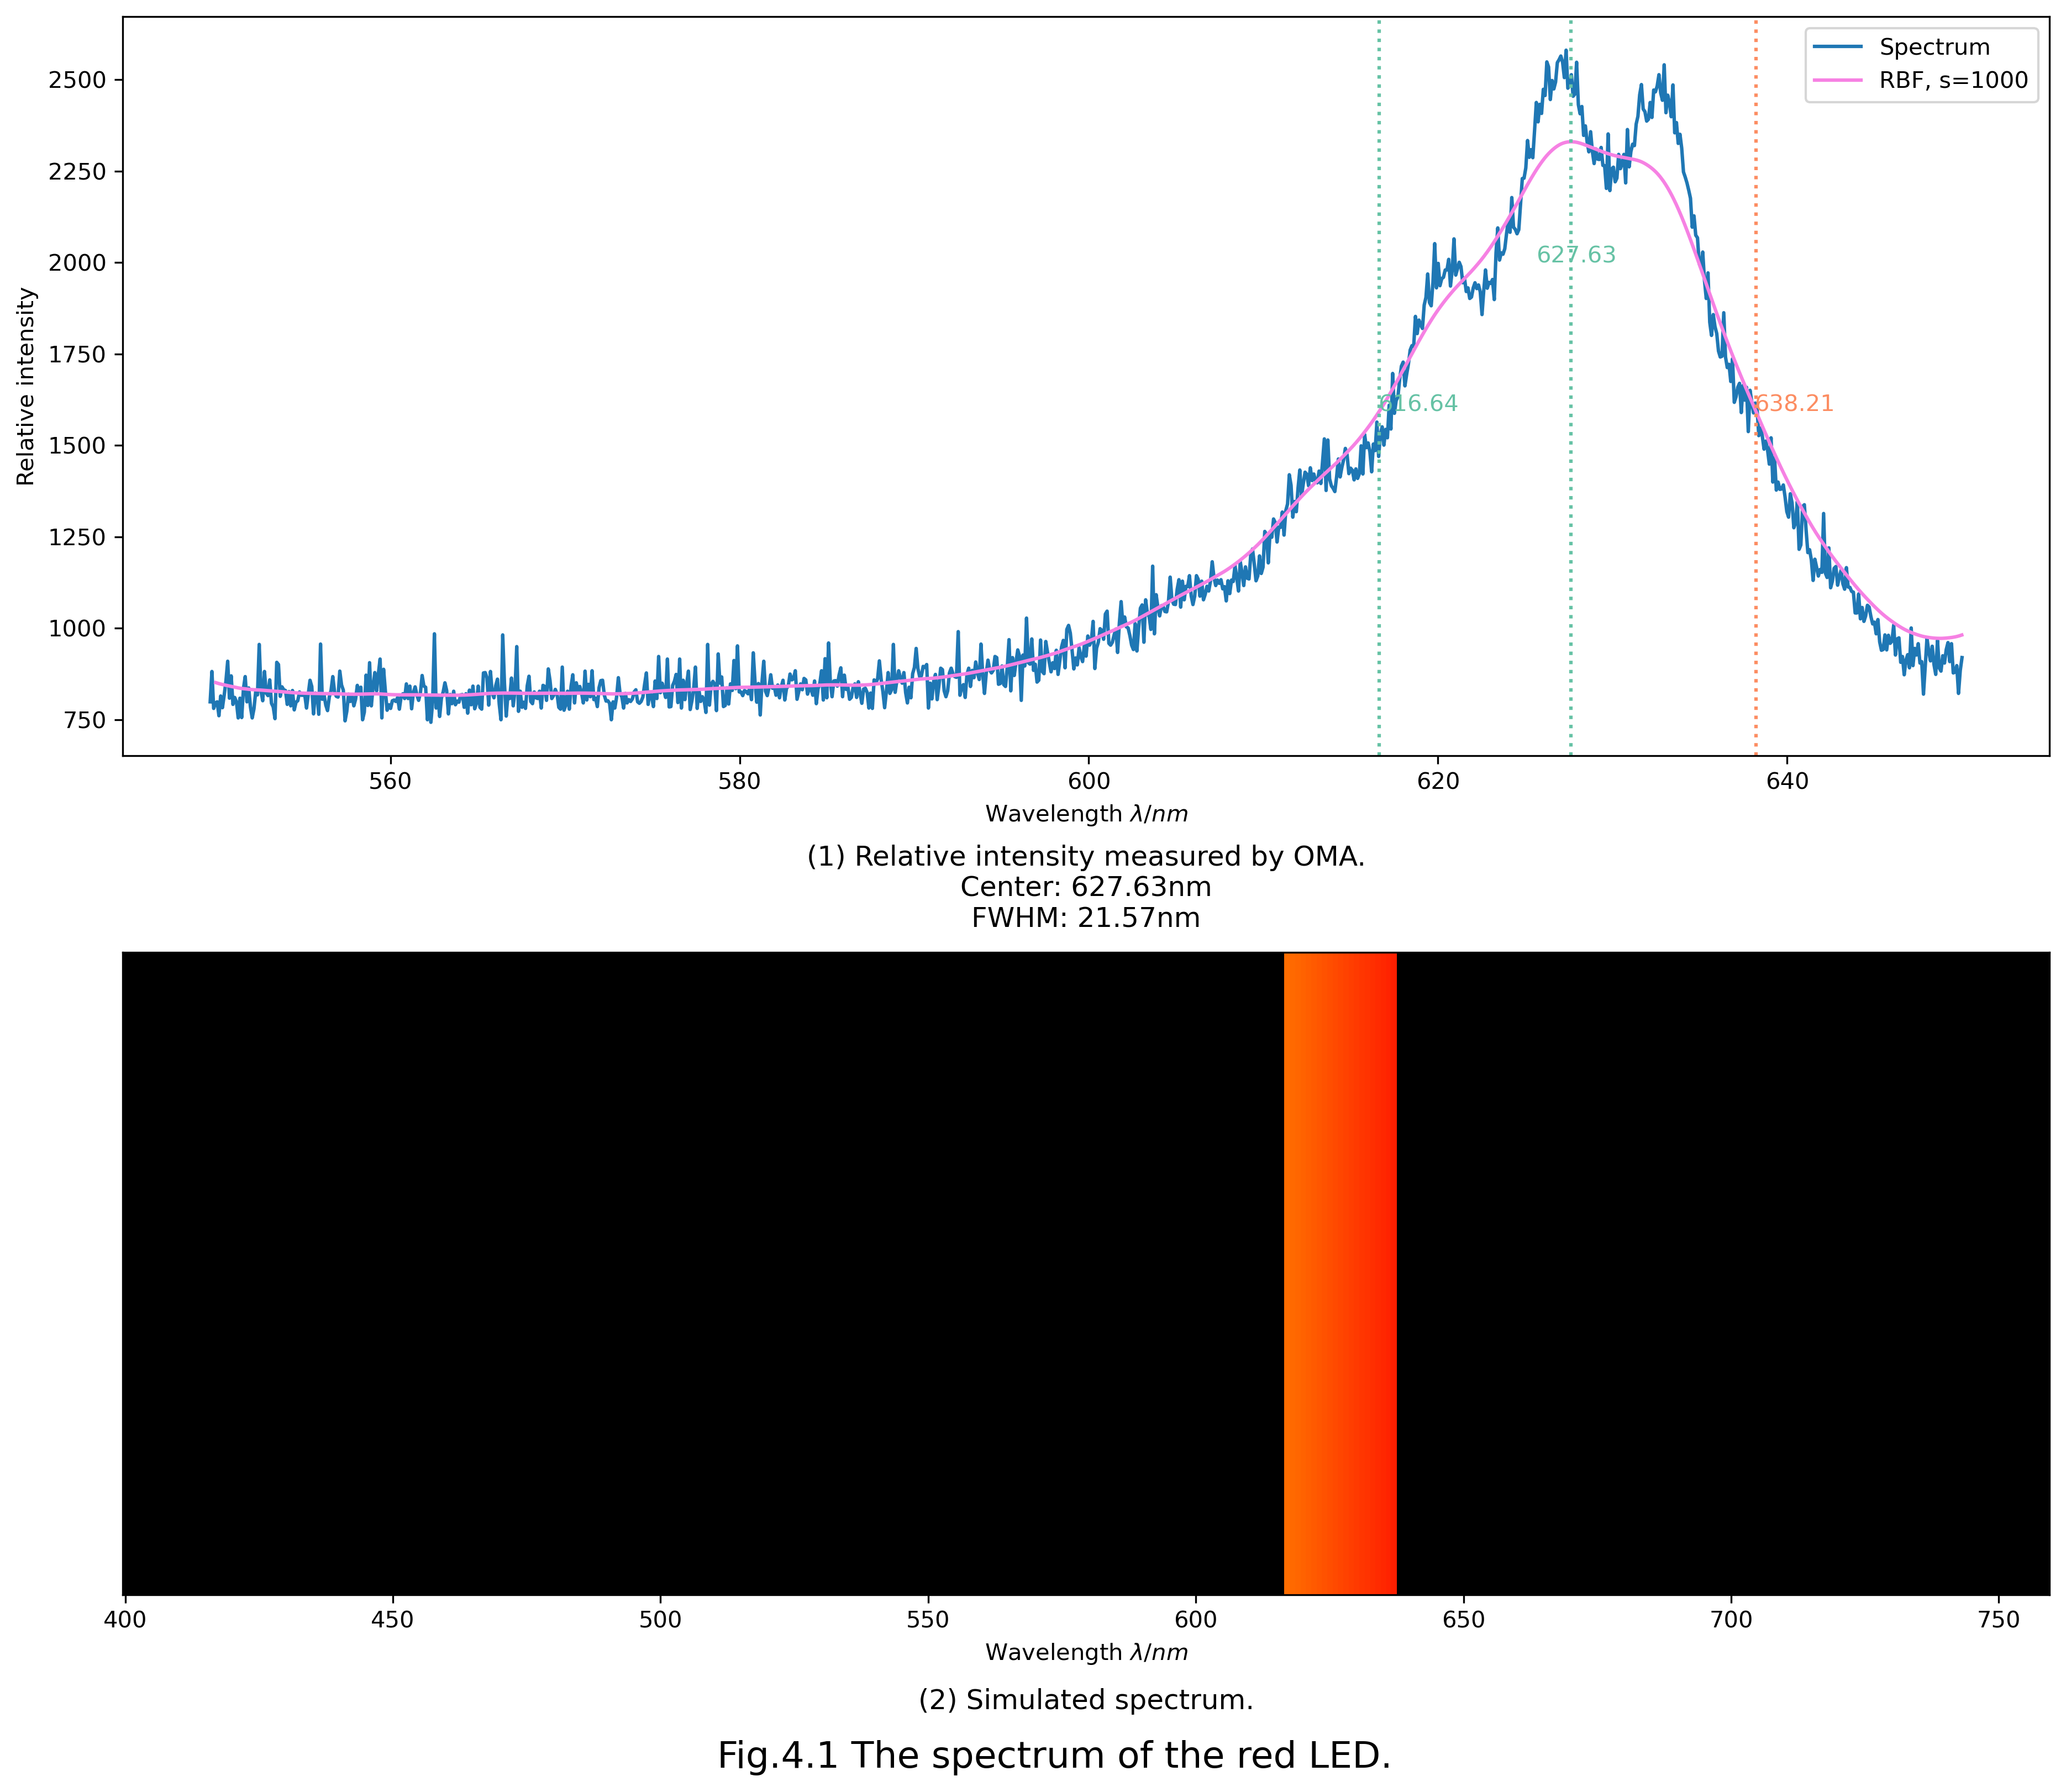
\includegraphics[width=0.33\textwidth]{attachments//Fig.4.1.png}
	}
	\subfloat[Blue]{\label{fig:4.2}
	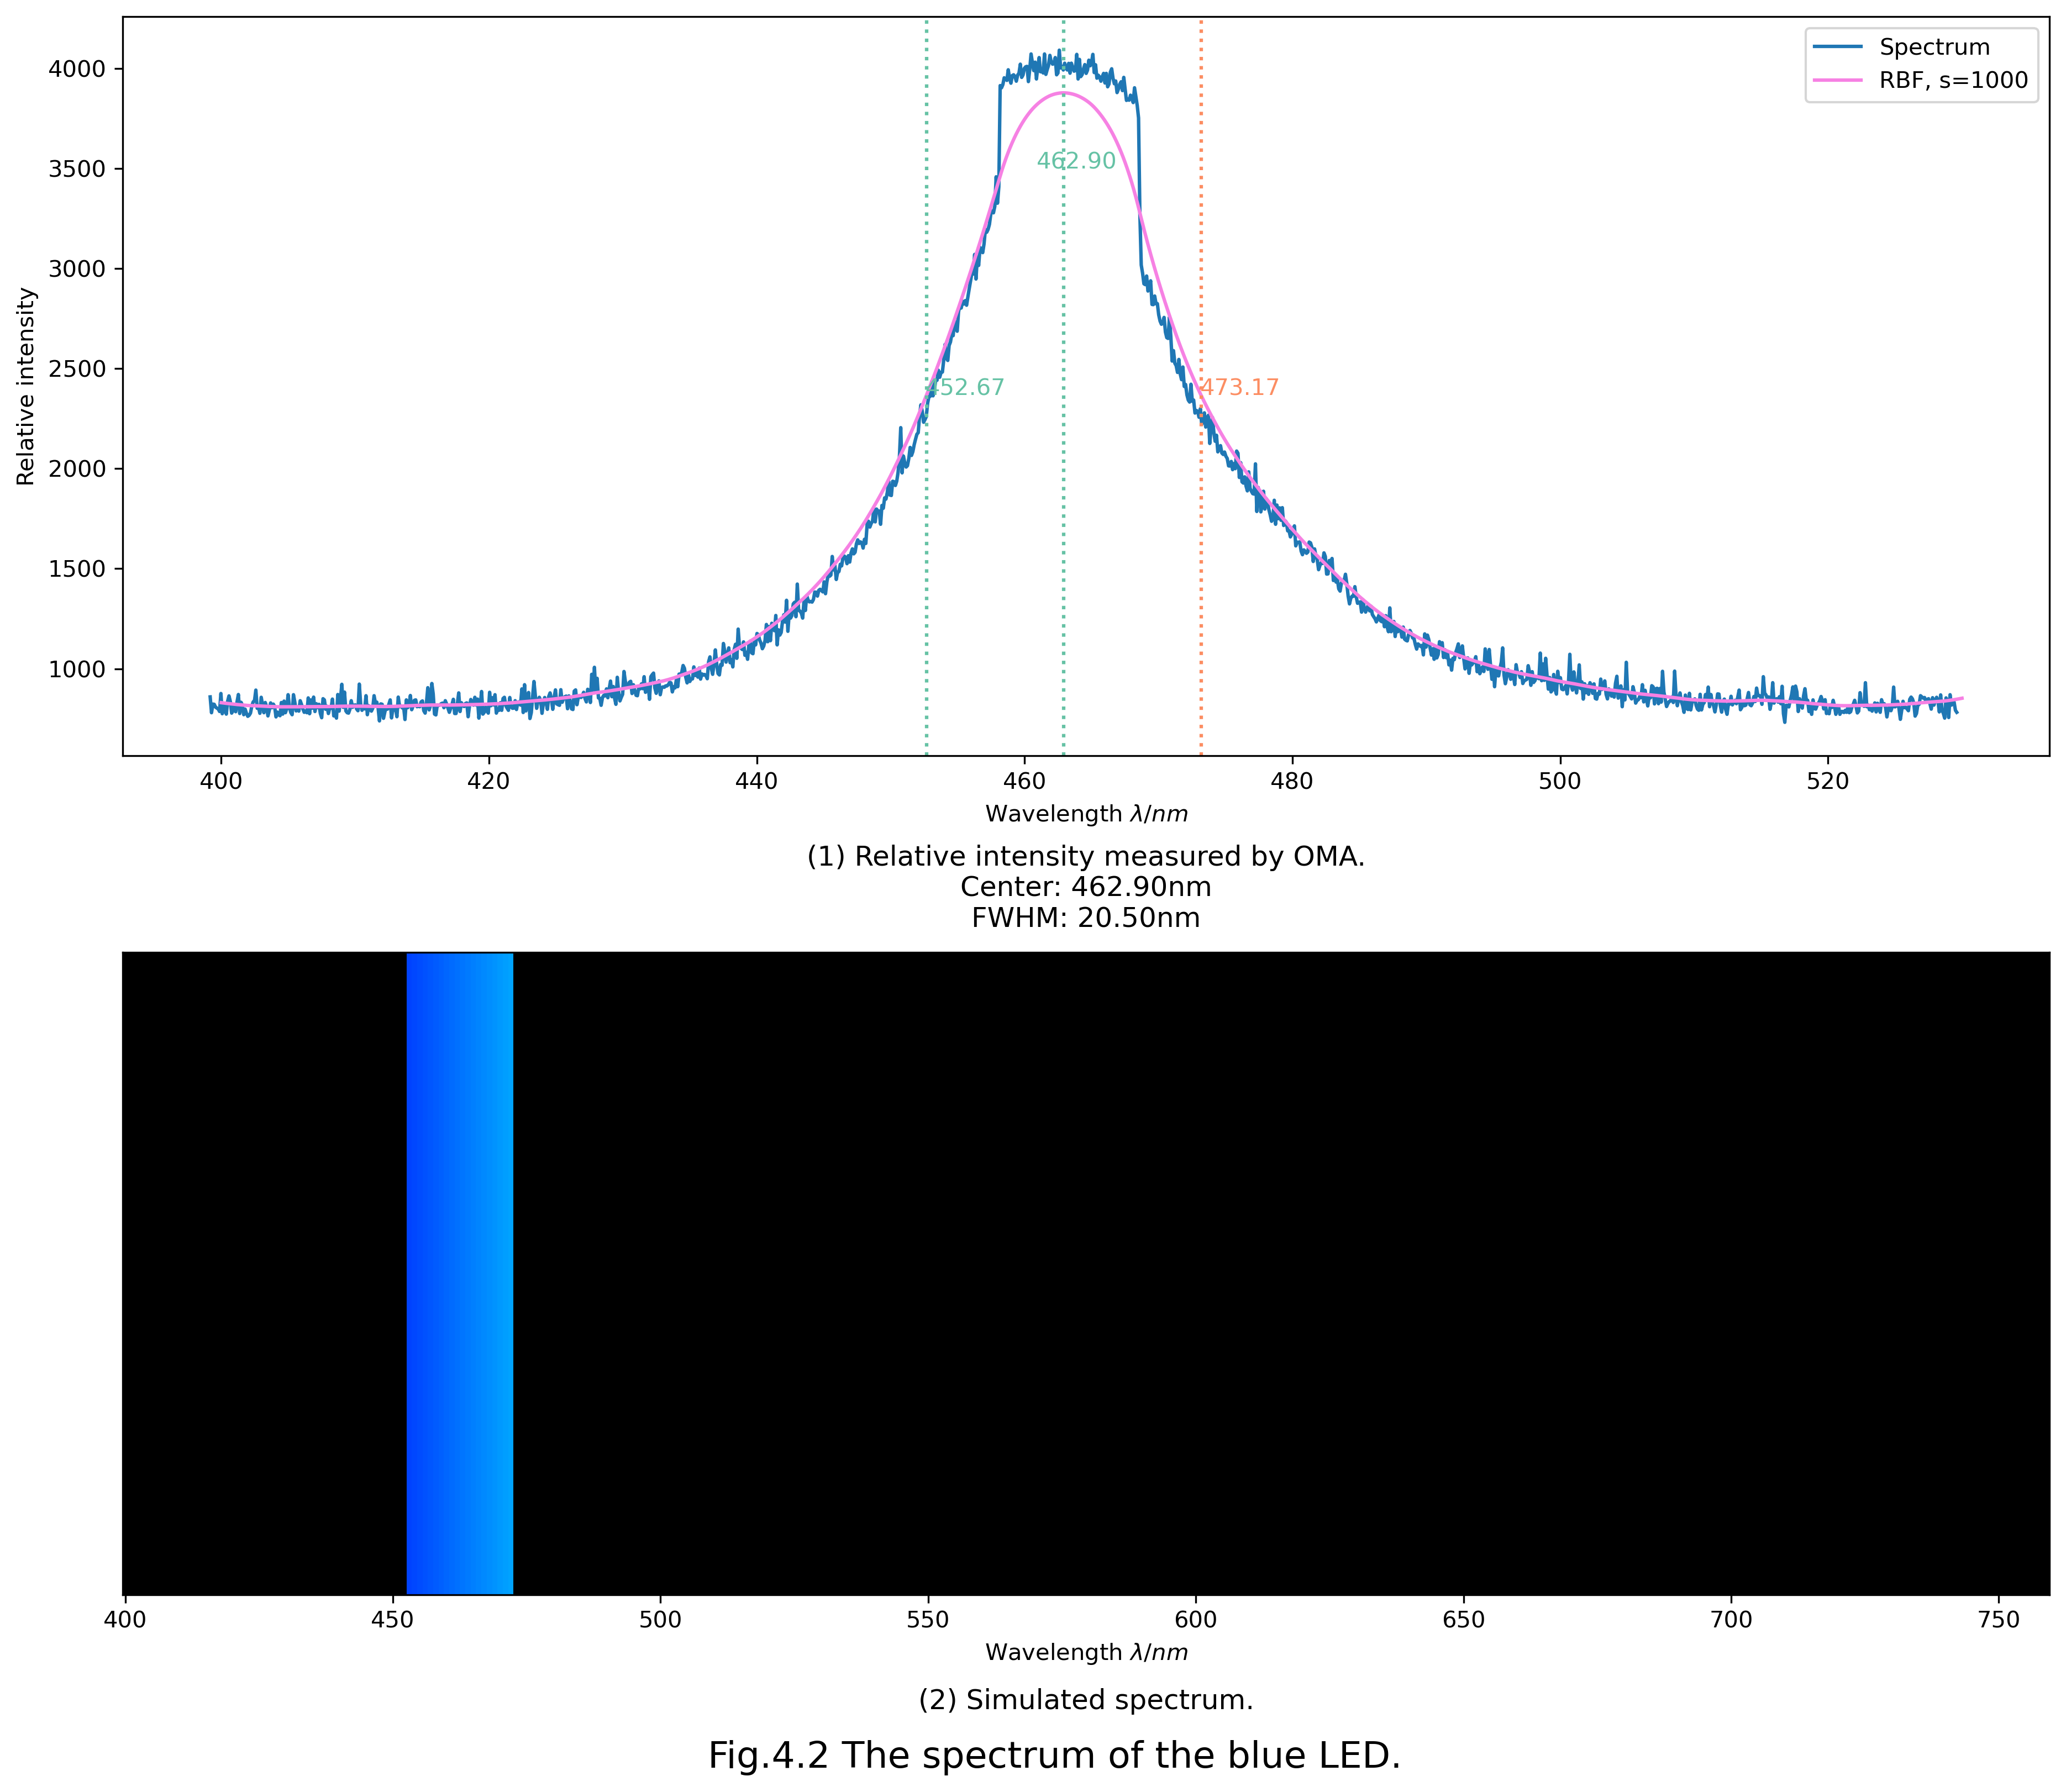
\includegraphics[width=0.33\textwidth]{attachments//Fig.4.2.png}
	}
	\subfloat[Green]{\label{fig:4.3}
	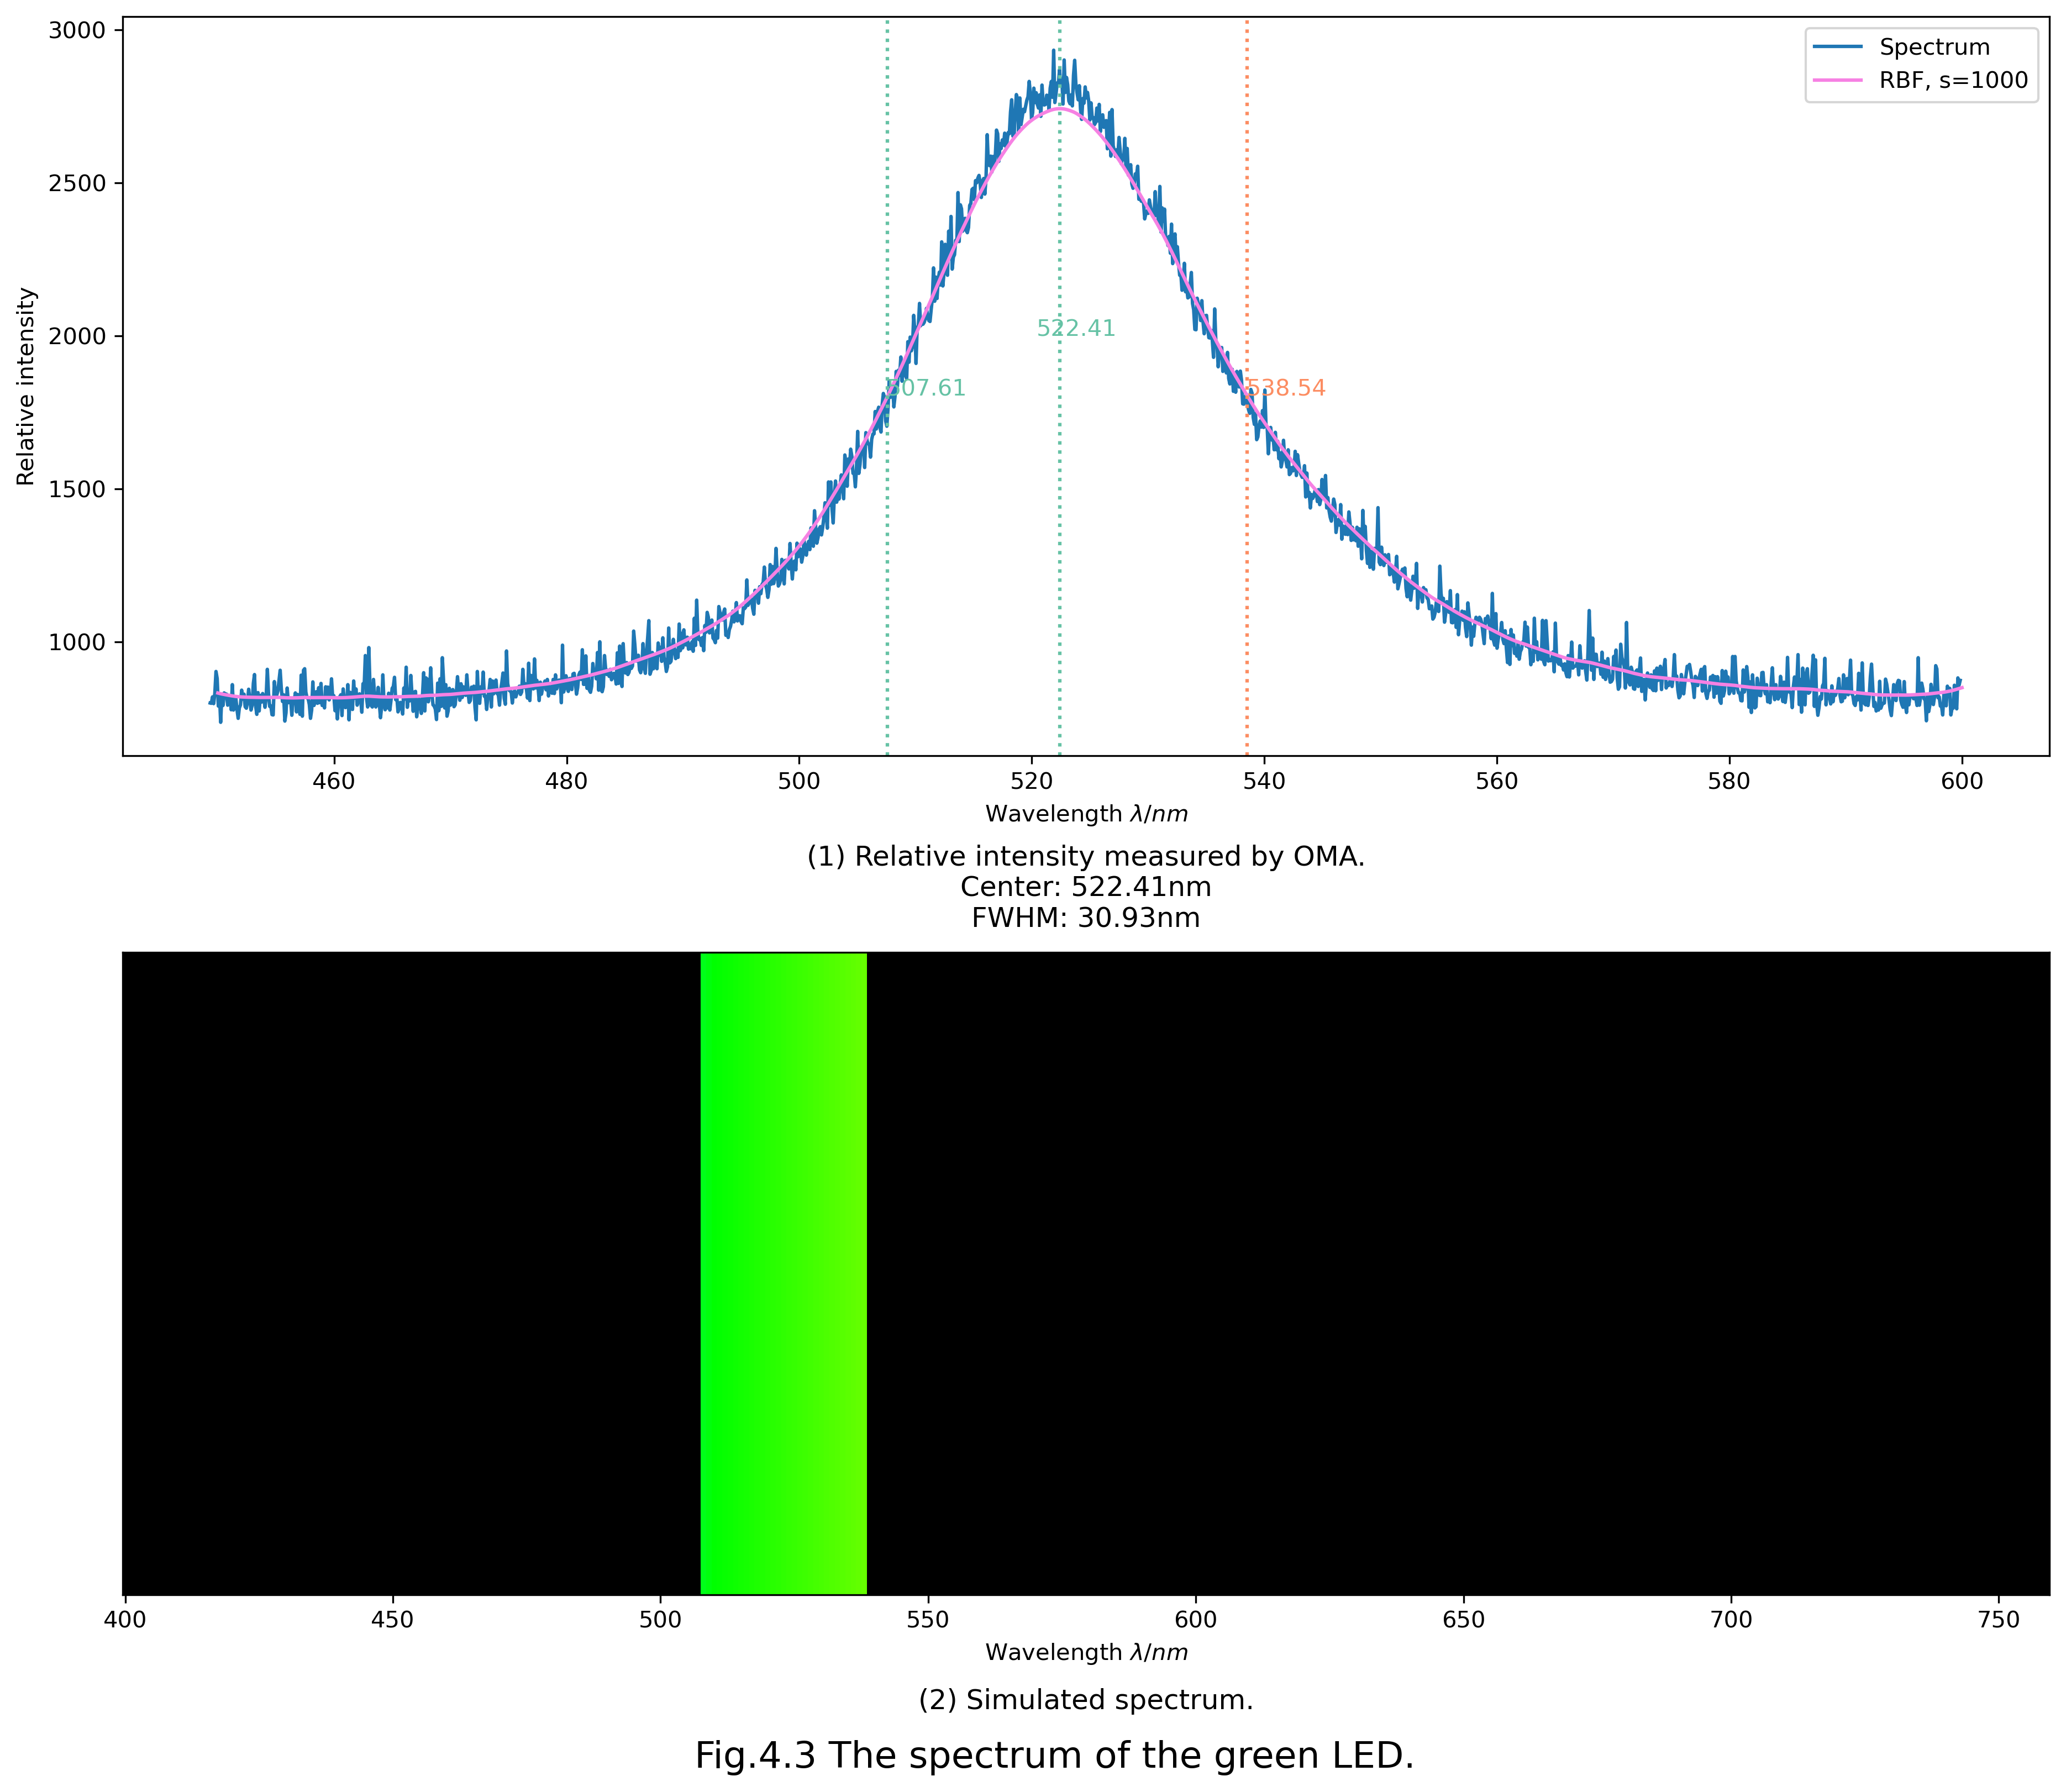
\includegraphics[width=0.33\textwidth]{attachments//Fig.4.3.png}
	}

	\subfloat[White]{\label{fig:4.4}
	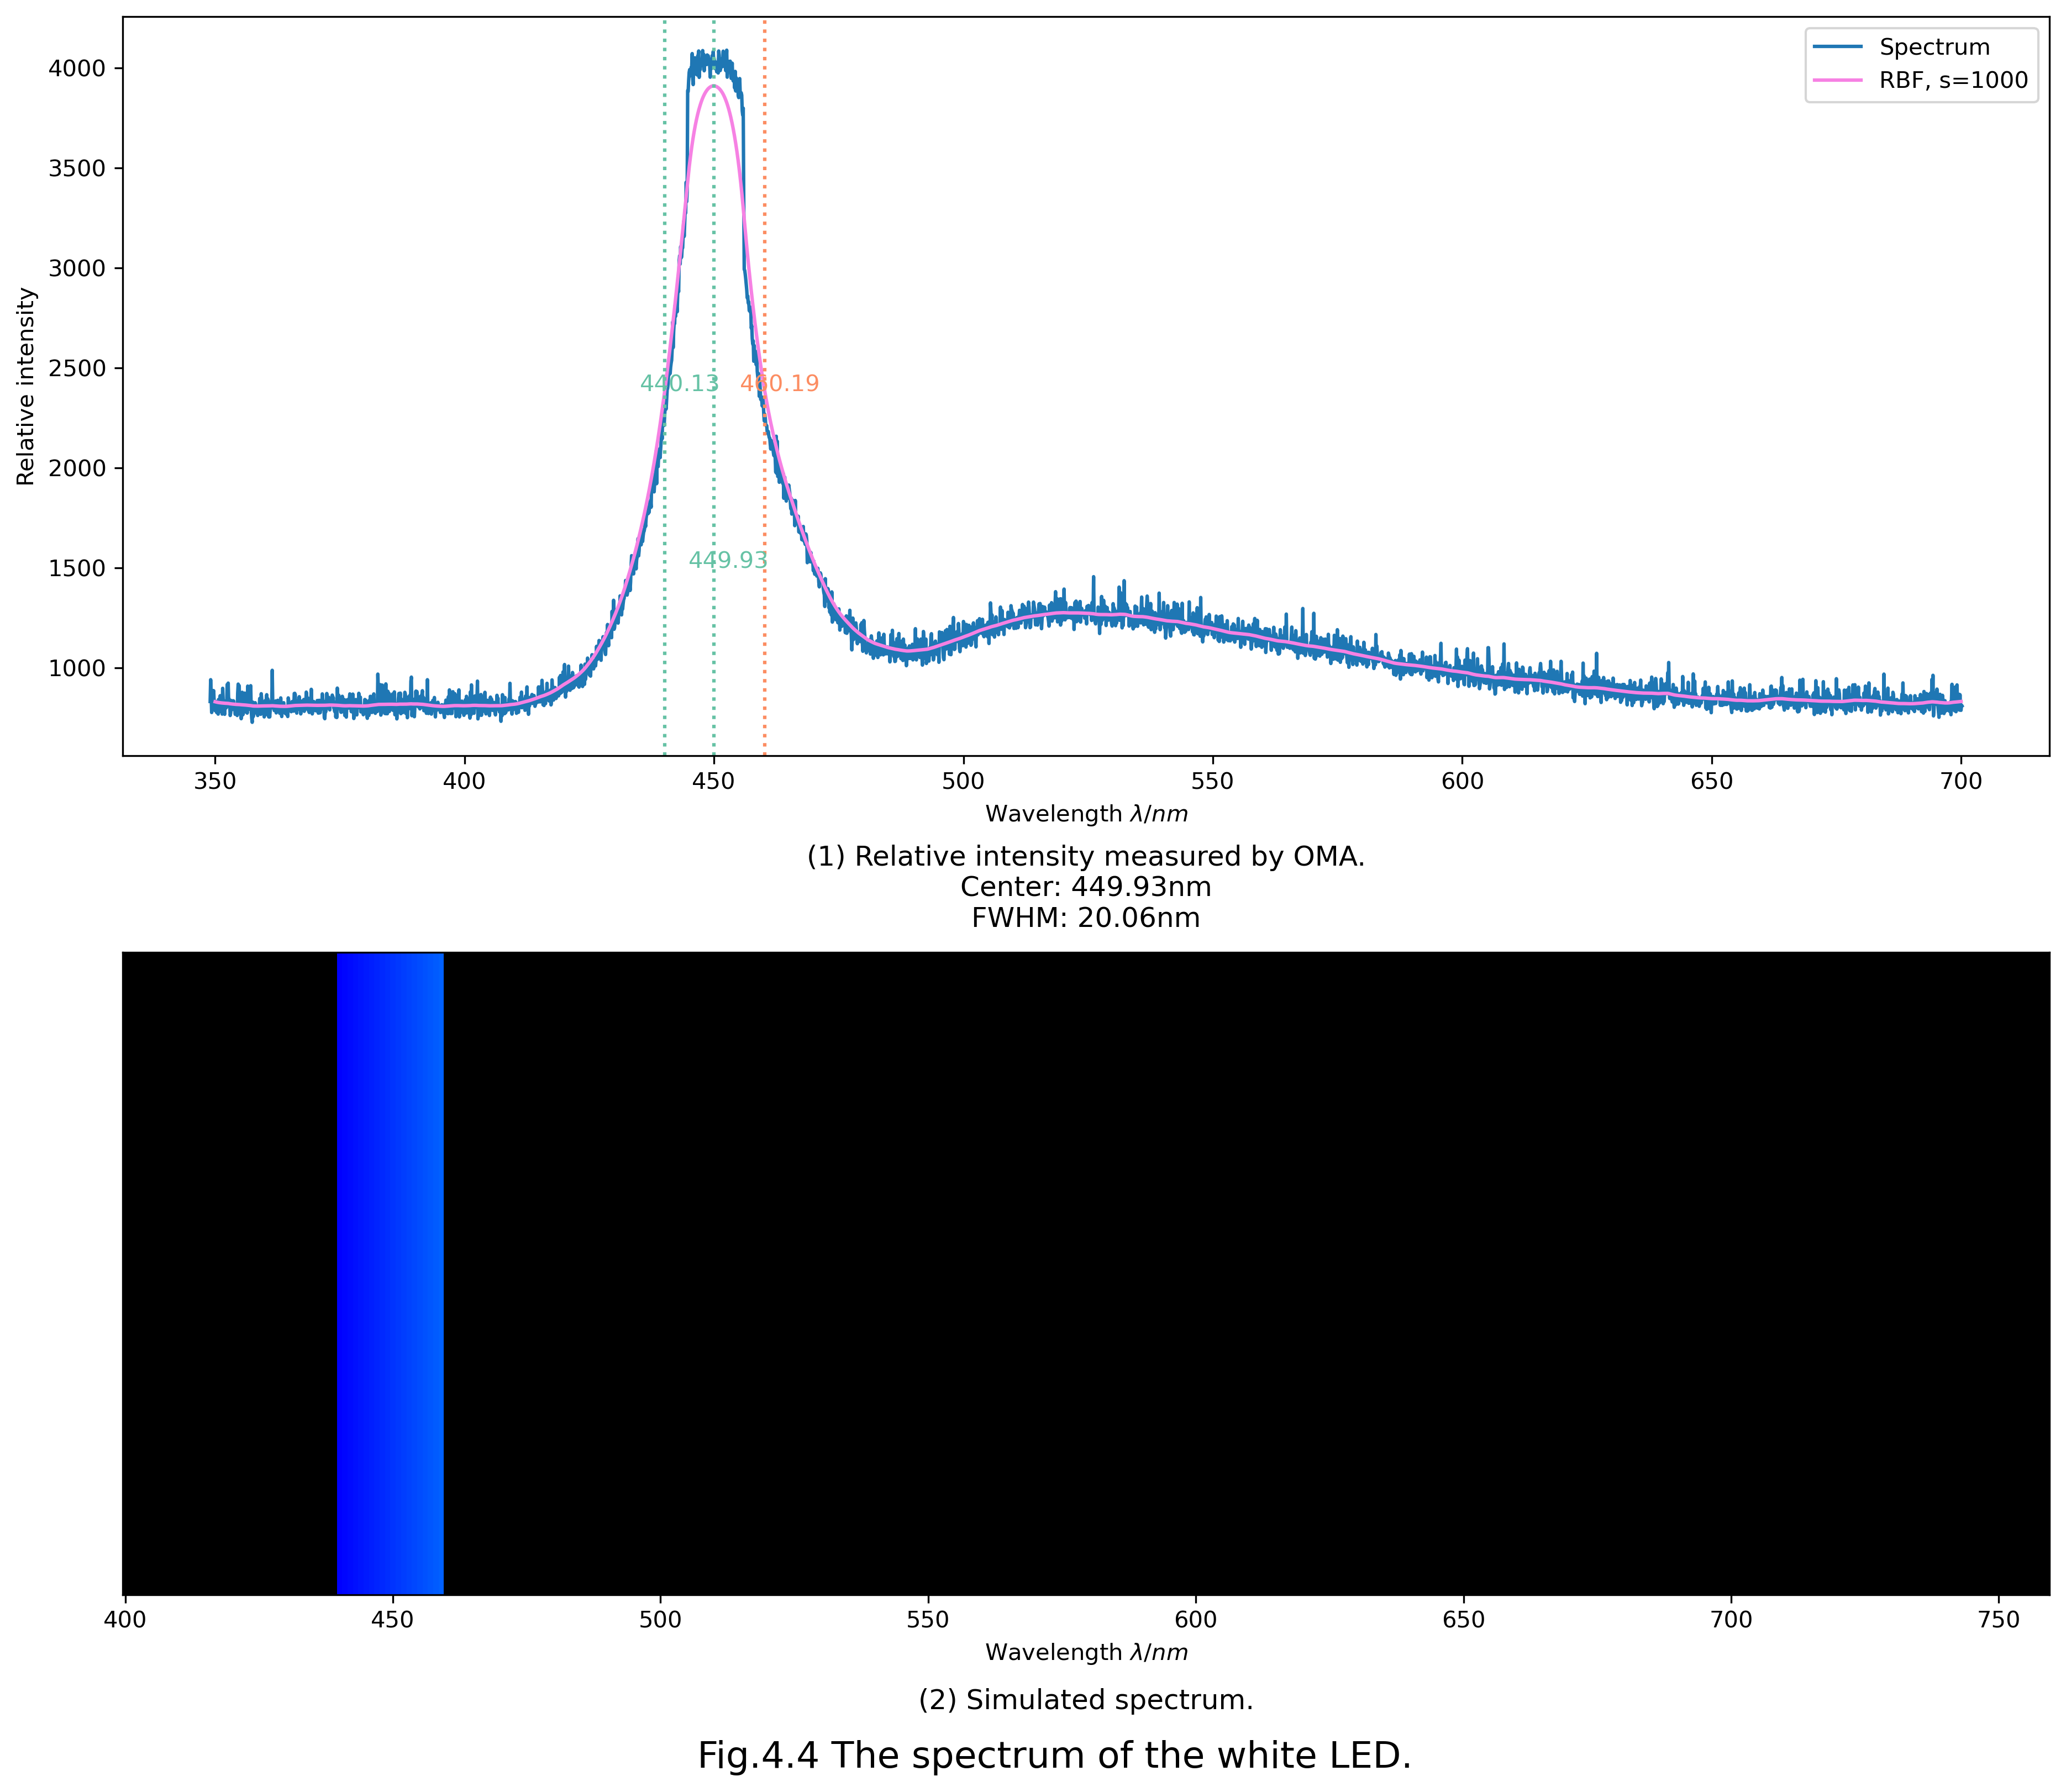
\includegraphics[width=0.33\textwidth]{attachments//Fig.4.4.png}
	}
	\subfloat[Yellow]{\label{fig:4.5}
	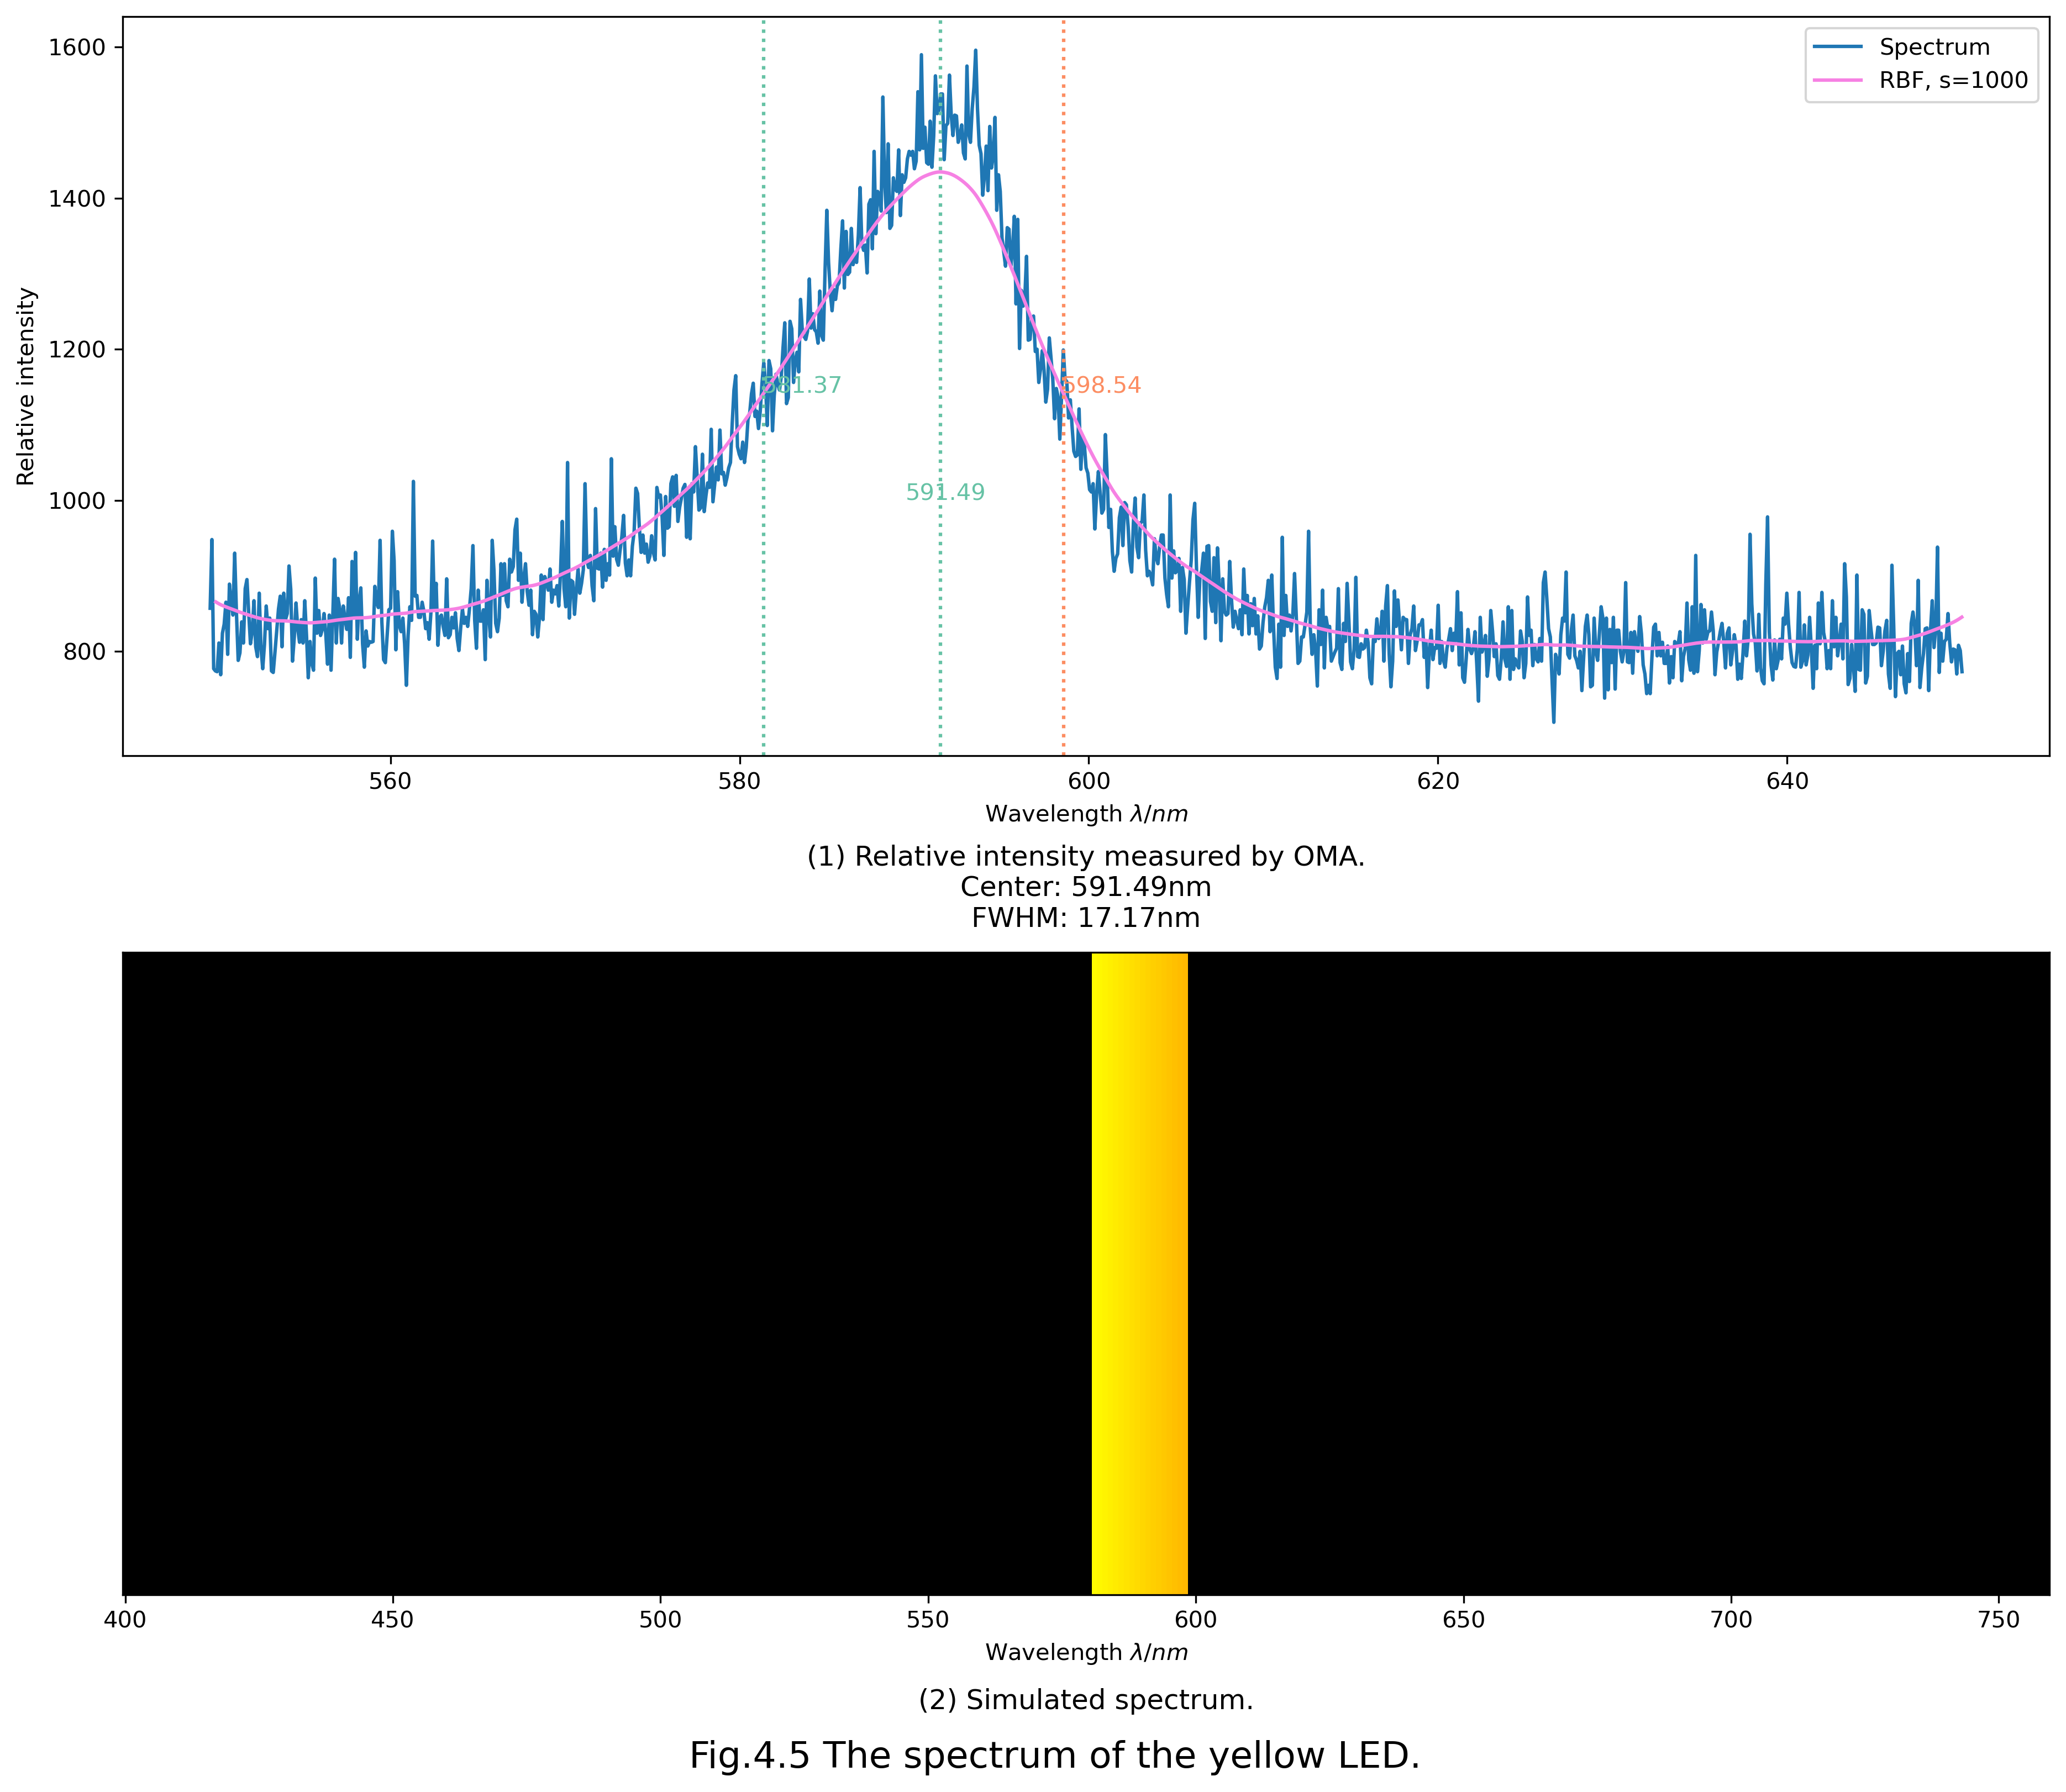
\includegraphics[width=0.33\textwidth]{attachments//Fig.4.5.png}
	}
	\caption{LED光谱}
	\label{fig:4}
\end{figure}

\begin{table}[htbp]
	\centering
	\begin{tabular}{ccc}
	\toprule
	LED &中心谱线/nm &半高宽/nm \\
	\midrule
	Red &$627.63$ &$21.57(616.64\sim 638.21)$ \\
	Blue &$462.90$ &$20.50(452.67\sim 473.17)$ \\
	Green &$522.41$ &$30.93(507.61\sim 538.54)$ \\
	White &$449.93$ &$20.06(440.13\sim 460.19)$ \\
	Yellow &$591.49$ &$17.17(581.37\sim 598.54)$ \\
	\bottomrule
    \end{tabular}
    \caption{\textbf{LED光谱}}
	\label{tab:4}
\end{table}

LED灯光谱均为连续谱,注意到白光LED光谱除在$450nm$附近有一显著增高外,在$480nm$后还有一个低幅增高后缓慢下降的隆起,这部分色光与显著隆起的蓝光区色光混合后使光线呈白色。

\subsubsection*{5. 溴钨灯光谱}
溴钨灯光谱如图\ref{fig:5}所示。溴钨灯光谱为连续谱,在可见光范围内均有分布,可见溴钨灯是工作在可见光范围内较好的光源。
同时注意到$650nm$附近有一个较强的突变。

\begin{figure}[htbp]
	\centering
	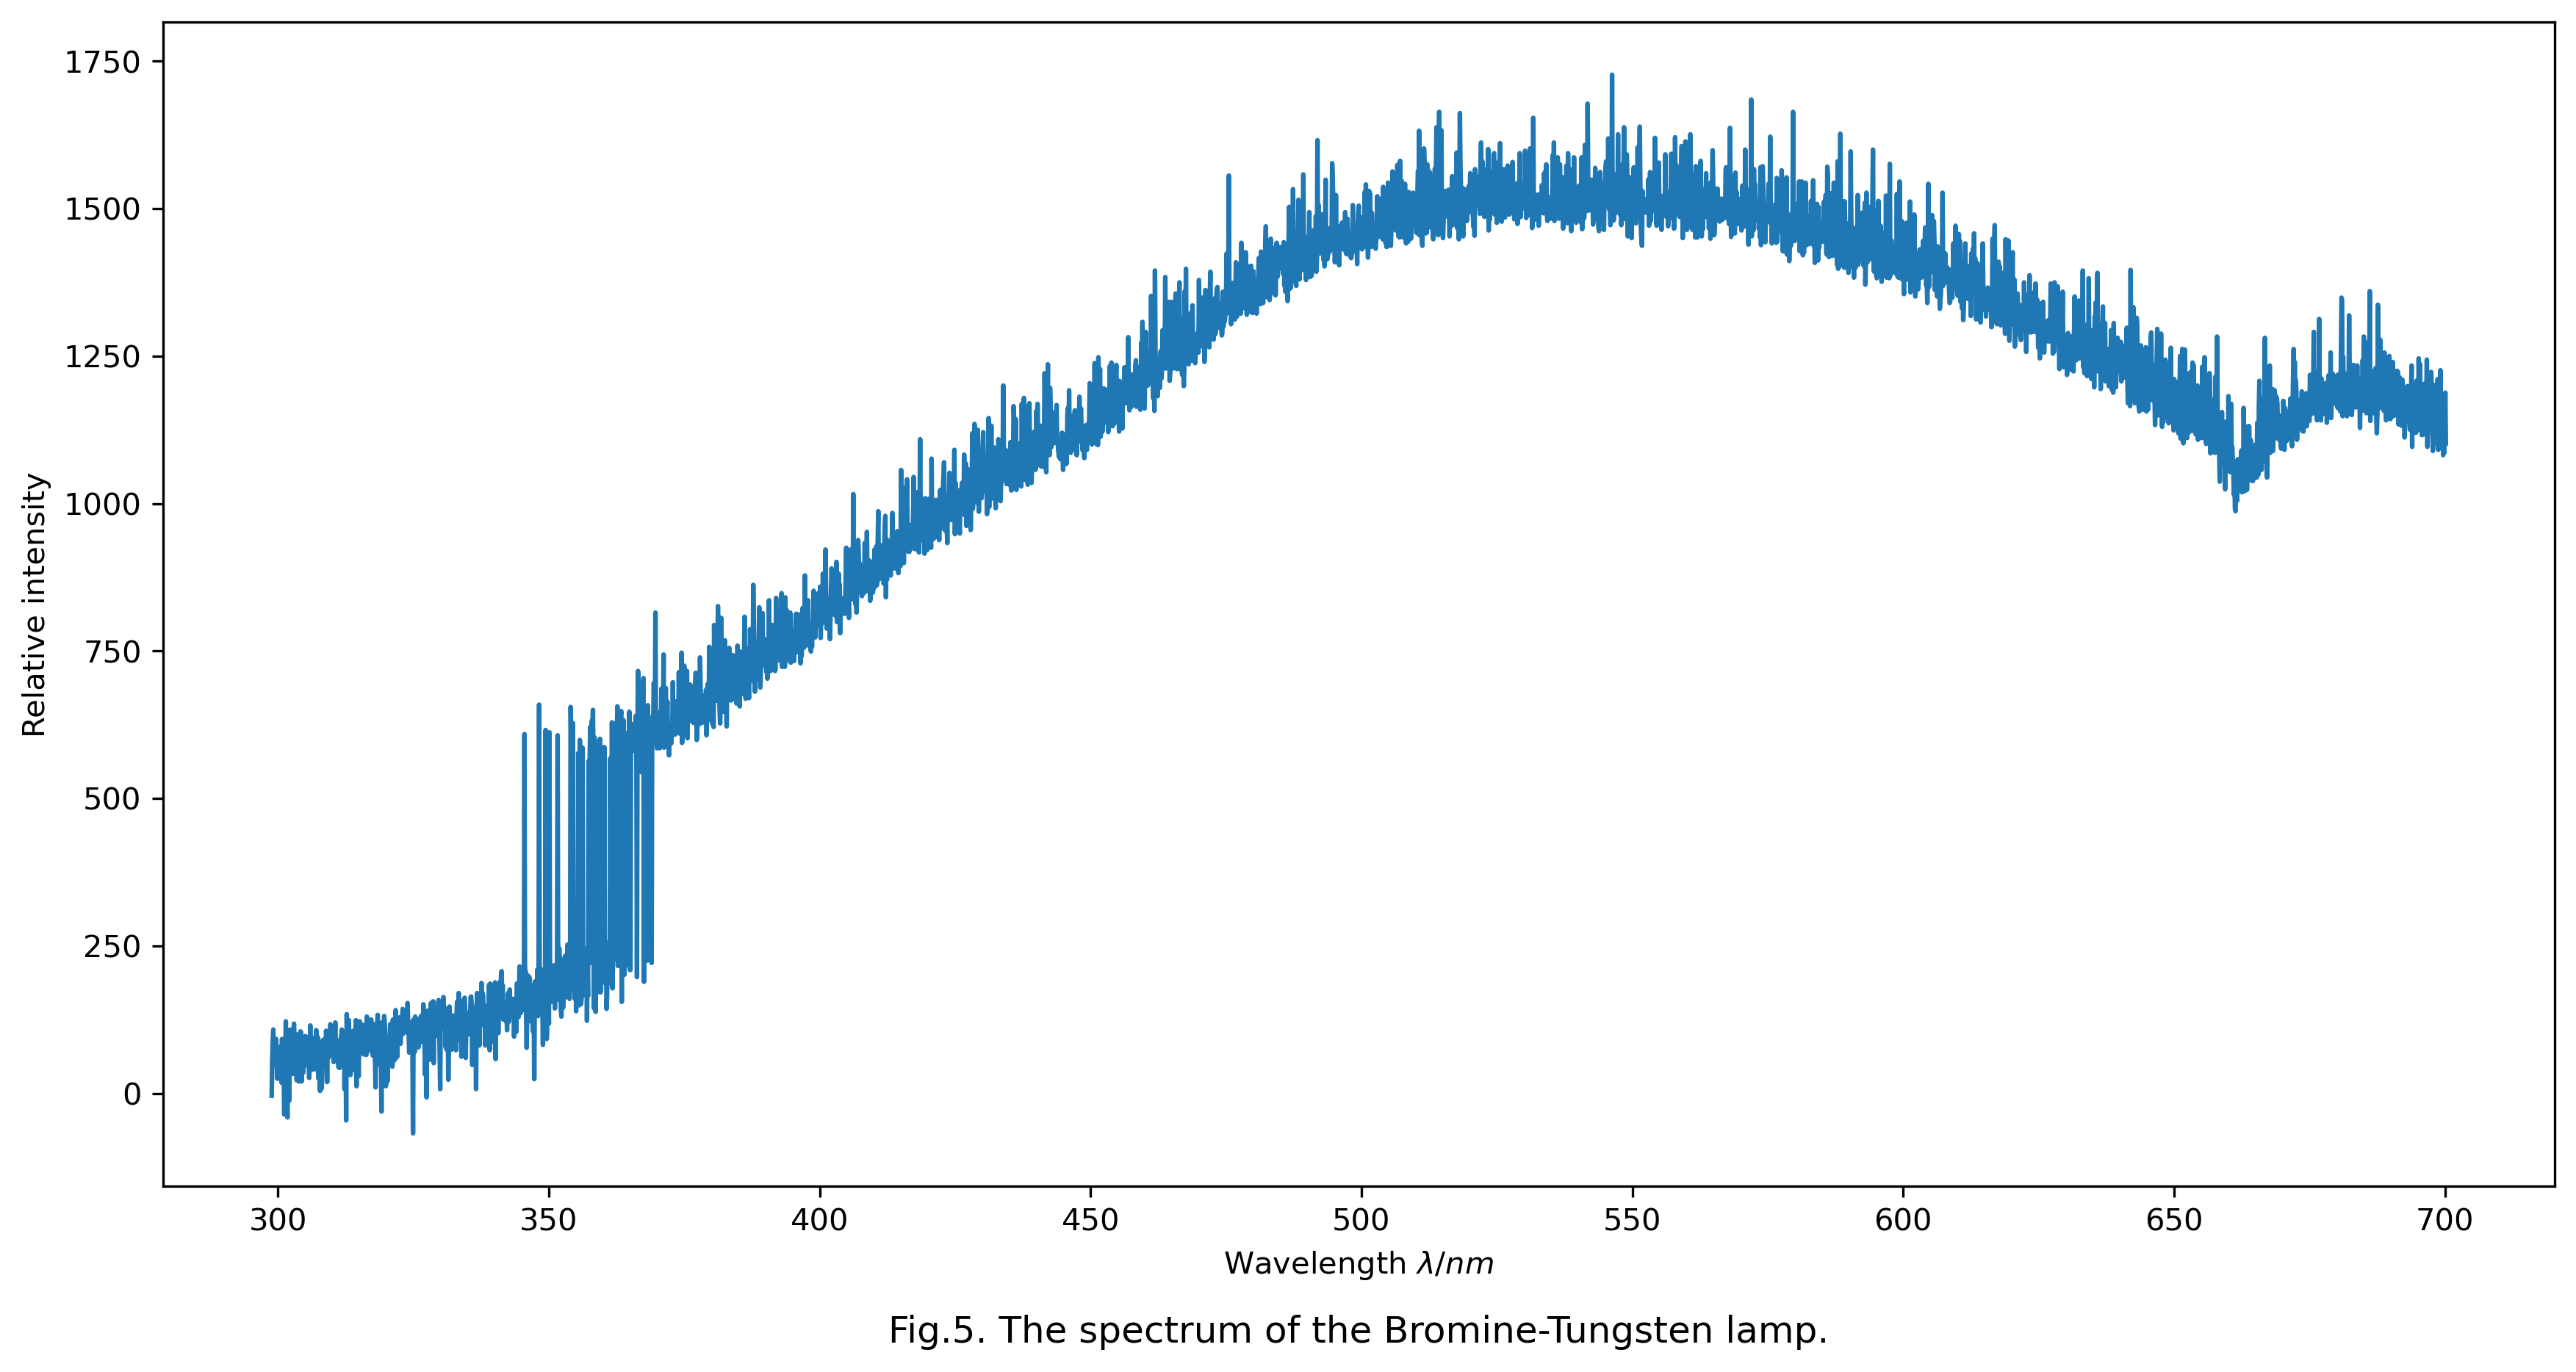
\includegraphics[width=0.8\textwidth]{attachments//Fig.5.png}
	\caption{溴钨灯光谱}
	\label{fig:5}
\end{figure}

\subsection*{【思考题】}
\subsubsection*{1. 钠原子光谱有哪些特征?从光谱图上如何判断各谱线所属线系?}
\begin{enumerate}[label=\arabic*.]
	\item 钠原子光谱为分立谱线,共有四个线系(主线系,锐线系,漫线系,基线系)
	\item 主线系只有钠双黄线在可见光区域内,其余谱线均在可见光波段外。
	\item 锐线系和漫线系除第一条谱线外,其余均在可见区。
	\item 基线系谱线全部在红外区。
	\item 因此可以根据各线系所在的光谱区域不同来区分不同线系。
\end{enumerate}

\subsection*{【项目源码】}
\href{https://github.com/Jeg-Vet/SYSU-PHY-EXP/tree/main/B13-Ultrasonic_grating}{SYSU-PHY-EXP/B13 Ultrasonic grating @Jeg-Vet(github.com)}

\end{document}

